% ===========================================================
% บทที่ 3: วิธีดำเนินการวิจัย
% ===========================================================

% -----------------------------------------------------------
\section{ภาพรวมกระบวนการวิจัย}
% -----------------------------------------------------------

หลักที่ผู้วิจัยยึดตลอดโครงงานคือ ให้ทั้งสองโมเดลใช้ข้อมูลและตัวชี้วัดชุดเดียวกัน
และระบุให้ชัดว่าสองโมเดลต่างกันตรงไหน ทั้งโครงสร้างของโมเดล ค่าสูญเสียส่วนเพิ่มของ HairFastGAN และ Epoch ที่มีไฟล์น้ำหนักให้เลือก
เพื่อให้ผลที่ต่างกันมาจากตัวโมเดลจริง ไม่ได้มาจากเงื่อนไขการทดลองที่ต่างกัน
งานทั้งหมดแบ่งเป็น 7 ขั้น ขั้นแรกคือเตรียมข้อมูล 169 ชุด แล้วแบ่งเป็นชุดฝึก ชุดตรวจสอบ และชุดทดสอบ
จากนั้นโหลดน้ำหนักทางการของ HairFastGAN (HFG) และ Barbershop (BS) มาเป็นจุดเริ่มต้น
แล้วปรับจูนเฉพาะส่วนที่ควบคุมสีและรายละเอียด โดยทดลองอัตราการเรียนรู้ 4 ชุด (เรียกแต่ละชุดว่า Trial) ชุดละ 30 รอบการฝึก (Epoch)
หลังจบแต่ละ Epoch จะวัดผลบนชุดตรวจสอบ แล้วใช้กติกาฉบับแก้ไขที่อธิบายในบทนี้
เลือกน้ำหนักที่เหมาะสมจากไฟล์น้ำหนักที่บันทึกไว้ (Checkpoint)
เมื่อเลือกได้แล้วจึงนำไปวัดผลบนชุดทดสอบเพียงครั้งเดียว
ขั้นต่อมาคือเติมรายละเอียดด้วย Stable Diffusion
และขั้นสุดท้ายคือให้ผู้ใช้ 41 คนประเมินภาพโดยไม่รู้ชื่อโมเดล เพื่อตัดสินว่าจะใช้โมเดลใดบนเว็บ
แล้วจึงเปิดให้ทดลองใช้งานจริง 100 ครั้ง

ภาพที่~\ref{fig:overview} สรุปทั้ง 7 ขั้นไว้ในภาพเดียว ให้อ่านจากซ้ายไปขวาตามขั้นที่ 1--6
ส่วนขั้นที่ 7 อยู่ในแถวล่างสุด ในคอลัมน์ของแต่ละขั้น แถวบนเป็นของ HairFastGAN และแถวล่างเป็นของ Barbershop
สีของกรอบบอกประเภทของงาน กรอบสีน้ำเงินคือส่วนเดิมของโมเดลที่ล็อกไว้ (ไม่ปรับน้ำหนัก)
กรอบสีส้มเส้นประคือส่วนที่ผู้วิจัยฝึกเพิ่ม กรอบสีเขียวคือขั้นขัดเกลาที่ผู้วิจัยเพิ่มเข้าไป
และกรอบสีม่วงคือการวัดผลและการเลือก
ตัวเลขในกรอบเป็นผลจริงของขั้นนั้น เช่น คะแนนของ Checkpoint ที่เลือก
ผู้อ่านจึงใช้ภาพนี้เป็นแผนที่ย้อนกลับมาดูได้ระหว่างอ่านบทที่ 3 และบทที่ 4

\begin{figure}[!htbp]
\centering
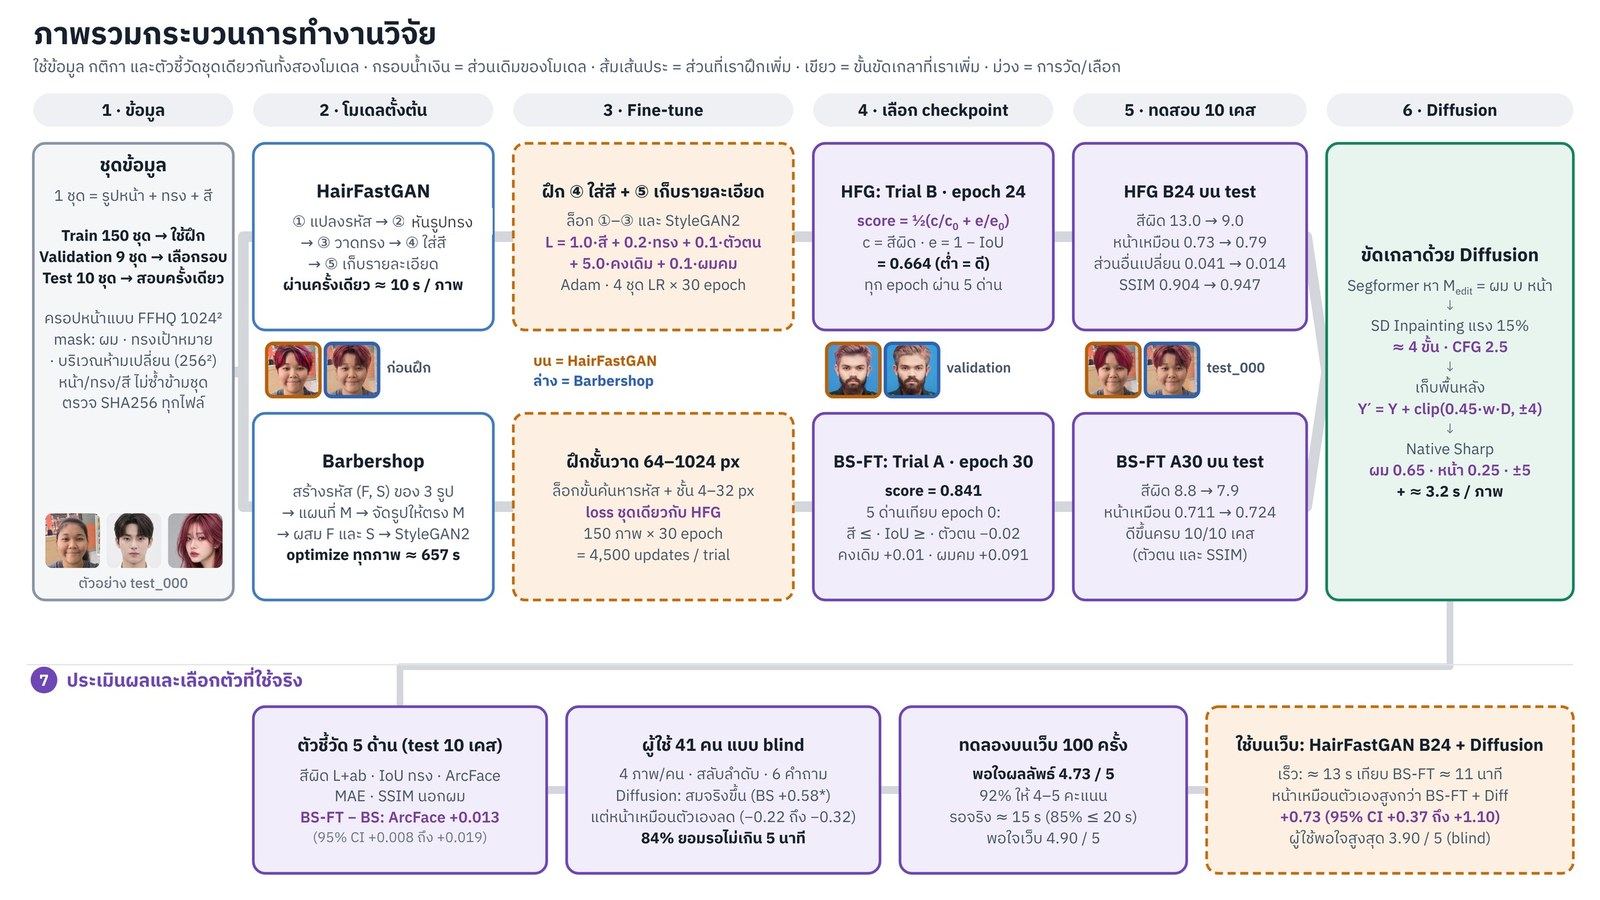
\includegraphics[width=\textwidth]{images/fig_overview.jpg}
\caption{ภาพรวมกระบวนการวิจัย ตั้งแต่ข้อมูล การปรับจูน การเลือก Checkpoint การทดสอบ
การขัดเกลาด้วย Diffusion จนถึงการคัดเลือกโมเดลสำหรับเว็บแอปพลิเคชัน}
\label{fig:overview}
\par\vspace{3pt}{\footnotesize\raggedright หมายเหตุ: HFG = HairFastGAN, BS = Barbershop, BS-FT (Barbershop-FT) = Barbershop ที่ปรับจูนแล้ว (Fine-tuned), B24 = น้ำหนักของ Trial B Epoch 24, A30 = น้ำหนักของ Trial A Epoch 30, IoU = Intersection over Union (สัดส่วนพื้นที่ผมที่ทับกัน), MAE = Mean Absolute Error (ค่าความคลาดเคลื่อนสัมบูรณ์เฉลี่ย)\par}
\end{figure}

% -----------------------------------------------------------
\section{ชุดข้อมูล}
% -----------------------------------------------------------

ข้อมูลหนึ่งชุดมี 3 ภาพ แต่ละภาพมีหน้าที่ต่างกัน ภาพใบหน้าคือภาพของคนที่จะเปลี่ยนผมให้
ทุกอย่างในภาพนี้ยกเว้นผมต้องคงเดิม ทั้งใบหน้า ผิว เสื้อผ้า และฉากหลัง
ภาพอ้างอิงทรงผมใช้เฉพาะรูปทรงของผม และภาพอ้างอิงสีผมใช้เฉพาะสีของผม
ภาพที่~\ref{fig:stage1_inputs} เป็นตัวอย่างข้อมูลหนึ่งชุด จากซ้ายไปขวาคือภาพใบหน้า ภาพทรงผม และภาพสีผม
เครื่องหมายบวกระหว่างภาพหมายถึงทั้งสามภาพถูกใช้ร่วมกันเพื่อสร้างภาพผลลัพธ์หนึ่งภาพ
จะเห็นว่าภาพทรงผมกับภาพสีผมเป็นคนละคนกันได้ ซึ่งทำให้งานยากขึ้น

ก่อนใช้งาน ภาพทุกภาพถูกครอปและจัดตำแหน่งใบหน้าให้ตรงกับรูปแบบของชุดข้อมูล Flickr-Faces-HQ (FFHQ)
ขนาด $1024 \times 1024$ พิกเซล เพราะ StyleGAN2 (Style-based Generative Adversarial Network รุ่นที่ 2) ของทั้งสองโมเดลถูกฝึกมากับภาพลักษณะนี้
ถ้าตำแหน่งตาหรือขนาดใบหน้าไม่ตรง โมเดลจะสร้างภาพเพี้ยนตั้งแต่ขั้นแรก
จากนั้นสร้างหน้ากาก (Mask) ขนาด $256 \times 256$ ไว้ 3 แบบ คือ หน้ากากผมเดิม
หน้ากากทรงผมเป้าหมาย และหน้ากากบริเวณที่ต้องคงเดิม
ซึ่งหมายถึงทุกพิกเซลที่ไม่ได้อยู่ในผมเดิมหรือผมใหม่ หน้ากากเหล่านี้ใช้ทั้งตอนคำนวณค่าสูญเสียและตอนวัดผล
ผู้วิจัยระวังไม่ให้ภาพเดียวกันไปอยู่ในหลายชุด เพราะถ้าภาพในชุดทดสอบเคยอยู่ในชุดฝึก
ผลทดสอบจะดีเกินจริง (เรียกว่าข้อมูลรั่ว หรือ Data Leakage) และได้ตรวจไฟล์ทุกไฟล์ด้วยค่าแฮช SHA-256
(Secure Hash Algorithm 256 บิต) ซึ่งเป็นรหัสประจำไฟล์ที่จะเปลี่ยนทันทีถ้าไฟล์ถูกแก้
เพื่อยืนยันว่าไม่มีไฟล์ซ้ำข้ามชุดข้อมูล และข้อมูลไม่ถูกแก้ระหว่างการทดลอง

\begin{figure}[!htbp]
    \centering
    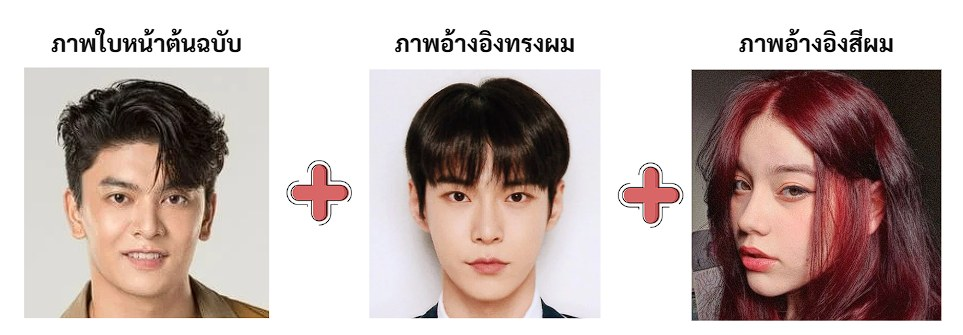
\includegraphics[width=0.85\textwidth]{images/stage1_inputs.jpg}
    \caption{ตัวอย่างข้อมูลนำเข้าหนึ่งชุด ได้แก่ ภาพใบหน้าต้นฉบับ ภาพอ้างอิงทรงผม และภาพอ้างอิงสีผม}
    \label{fig:stage1_inputs}
\end{figure}

ตารางที่~\ref{tab:dataset} แสดงว่าข้อมูล 169 ชุดถูกแบ่งอย่างไร และแต่ละส่วนมีไว้ทำอะไร
ชุดฝึก 150 ชุดเป็นชุดเดียวที่โมเดลได้เรียนรู้ ชุดตรวจสอบ 9 ชุดใช้ดูผลหลังจบแต่ละ Epoch
เพื่อเลือก Checkpoint และชุดทดสอบ 10 ชุดใช้ประเมิน Checkpoint ที่เลือกไว้แล้ว
อย่างไรก็ตาม ผู้วิจัยเคยประเมินโมเดลก่อนปรับจูนบนชุดทดสอบนี้ไปแล้วครั้งหนึ่งก่อนแก้กติกาการเลือก
ชุดทดสอบจึงไม่ใช่ชุดที่ไม่เคยถูกเปิดดูเลย
เหตุผลที่ต้องแยกชุดตรวจสอบออกจากชุดทดสอบคือ ถ้าใช้ชุดเดียวกันทั้งเลือกโมเดลและวัดผล
ผู้วิจัยอาจเผลอเลือกโมเดลที่บังเอิญเข้ากับข้อมูลชุดนั้น แล้วรายงานผลที่ดีเกินจริง

\begin{table}[!htbp]
\centering
\caption{การแบ่งชุดข้อมูล}
\label{tab:dataset}
\begin{tabular}{|L{3.8cm}|c|L{8.2cm}|}
\hline
\textbf{ชุดข้อมูล} & \textbf{จำนวนชุด} & \textbf{หน้าที่} \\ \hline
ชุดฝึก (Train) & 150 & ใช้ปรับน้ำหนักโมเดล เป็นชุดเดียวที่โมเดลเห็นระหว่างการฝึก \\ \hline
ชุดตรวจสอบ (Validation) & 9 & วัดผลหลังจบทุก Epoch เพื่อเลือก Checkpoint \\ \hline
ชุดทดสอบ (Test) & 10 & ล็อก Checkpoint ไว้ก่อน แล้ววัดผลเพียงครั้งเดียว \\ \hline
\textbf{รวม} & \textbf{169} & \\ \hline
\end{tabular}
\end{table}

% -----------------------------------------------------------
\section{เครื่องมือและสภาพแวดล้อม}
% -----------------------------------------------------------

โค้ดทั้งหมดเขียนด้วยภาษา Python โดยใช้ PyTorch สำหรับโมเดล GAN (Generative Adversarial Network)
และใช้ไลบรารี Hugging Face Diffusers กับ Transformers สำหรับ Stable Diffusion และ SegFormer (Segmentation Transformer)
การทดลองทุกขั้น รวมถึงการจับเวลา รันบน Google Colab ด้วยหน่วยประมวลผลกราฟิก (Graphics Processing Unit: GPU)
NVIDIA A100 หน่วยความจำ 40 GB เพื่อให้เวลาของทุกระบบเทียบกันได้
โมเดลที่นำมาใช้โดยไม่ได้ฝึกเอง ได้แก่ น้ำหนักทางการของ HairFastGAN และ Barbershop
(ซึ่งมี StyleGAN2 ที่ฝึกบน FFHQ อยู่ภายใน), BiSeNet (Bilateral Segmentation Network), ArcFace (Additive Angular Margin Loss),
CLIP (Contrastive Language-Image Pre-training), SegFormer-B2
และ Stable Diffusion แบบเติมภาพ (Inpainting) รุ่น Realistic Vision v5.1
ทุกการทดลองใช้ค่าเริ่มต้นของตัวสุ่ม (Seed) 3407 และบันทึกค่าแฮชของ Checkpoint ข้อมูล และการตั้งค่า
เพื่อให้รันซ้ำแล้วได้ผลเดิม

% -----------------------------------------------------------
\section{ขั้นตอนการทำงานของ Barbershop-FT (Barbershop ที่ปรับจูนแล้ว)}
\label{sec:pipe_bs}
% -----------------------------------------------------------

Barbershop (หลักการอยู่ในหัวข้อที่~\ref{sec:barbershop}) ทำงาน 6 ขั้น
ห้าขั้นแรกเป็นการค้นหารหัสของภาพ ซึ่งเป็นส่วนเดิมของโมเดลที่ผู้วิจัยไม่ได้แก้
ขั้นที่ 6 คือการวาดภาพด้วย StyleGAN2 ซึ่งเป็นขั้นเดียวที่มีน้ำหนักให้ปรับจูน
ในเล่มนี้เรียก Barbershop ที่ปรับจูนแล้วว่า Barbershop-FT (BS-FT)
ภาพที่~\ref{fig:pipe_bs} แสดงทั้งระบบเป็น 3 แถว แถวแรกคือ 6 ขั้นของ Barbershop-FT
ตั้งแต่ภาพนำเข้าจนได้ภาพจาก GAN แถวที่สองคือขั้นขัดเกลาด้วย Diffusion ที่ต่อท้าย
และแถวที่สามคือวิธีปรับจูน ในแต่ละกล่องมีสูตรและค่าที่ใช้จริงกำกับไว้
ซึ่งจะอธิบายทีละขั้นต่อไปนี้

\begin{figure}[!htbp]
\centering
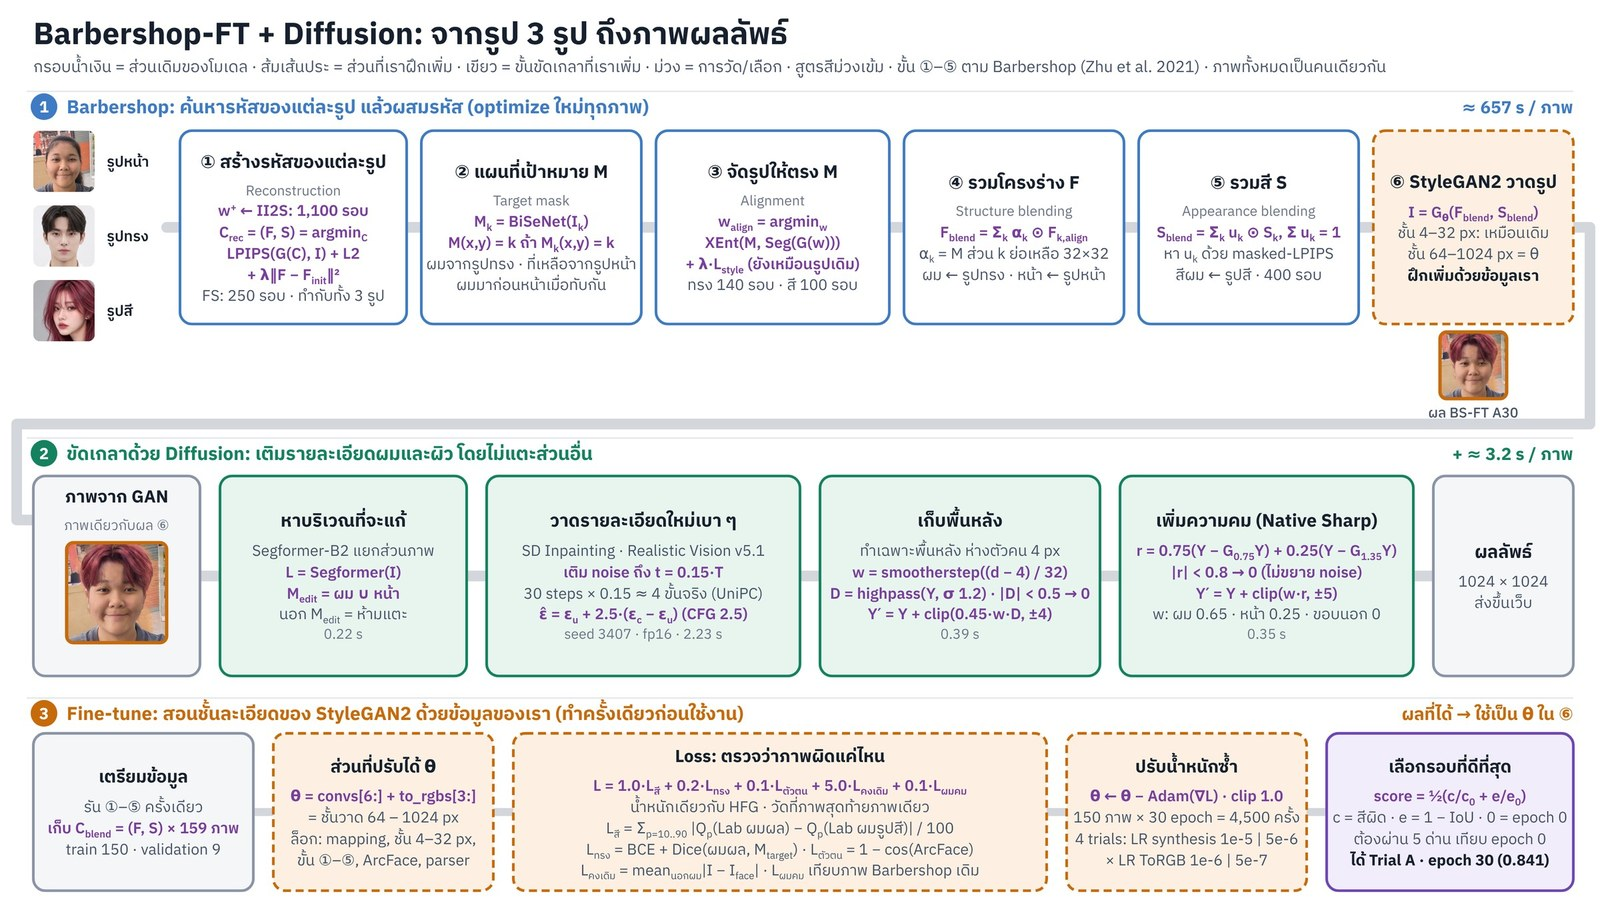
\includegraphics[width=\textwidth]{images/fig_pipeline_bs.jpg}
\caption{ขั้นตอนการทำงานของ Barbershop-FT + Diffusion ตั้งแต่ภาพนำเข้า 3 ภาพ
จนถึงภาพผลลัพธ์ พร้อมส่วนที่ปรับจูน}
\label{fig:pipe_bs}
\par\vspace{3pt}{\footnotesize\raggedright หมายเหตุ: BS-FT (Barbershop-FT) = Barbershop ที่ปรับจูนแล้ว (Fine-tuned), LPIPS = Learned Perceptual Image Patch Similarity, StyleGAN2 = Style-based Generative Adversarial Network รุ่นที่ 2, BiSeNet = Bilateral Segmentation Network, SegFormer = Segmentation Transformer\par}
\end{figure}

ขั้นที่ 1 คือการแปลงภาพกลับเป็นรหัส (GAN Inversion)
StyleGAN2 วาดภาพได้จากรหัสเท่านั้น จึงต้องหาก่อนว่ารหัสแบบใดที่เมื่อวาดออกมาแล้วได้ภาพนั้น
Barbershop ทำโดยตรึง StyleGAN2 ไว้ แล้วค่อย ๆ ปรับรหัส $w$ โดยเริ่มจากรหัสเฉลี่ย
จนภาพที่วาดได้ใกล้ภาพจริงที่สุด ตามสมการที่~(\ref{eq:m_inv})
การค้นหาเริ่มในพื้นที่ $W^{+}$ ด้วยวิธี II2S (Improved Image2StyleGAN) 1,100 รอบ แล้วค้นต่อในพื้นที่ $FS$ อีก 250 รอบ
ด้วยอัตราการเรียนรู้ 0.01 โดยทำแบบนี้กับทั้ง 3 ภาพ
ผลที่ได้ของแต่ละภาพคือ $F$ ซึ่งเป็นคุณลักษณะขนาด $32 \times 32 \times 512$ ที่เก็บโครงร่างของภาพ
และ $S$ ซึ่งเป็นสไตล์ของชั้นที่เหลือที่เก็บสีและพื้นผิว
ขั้นนี้ใช้เวลามากที่สุดของ Barbershop
\begin{equation}
w^{*} = \arg\min_{w} \; \mathrm{LPIPS}\left(G(w), I\right) + \lambda \left\lVert G(w) - I \right\rVert_2^2
\label{eq:m_inv}
\end{equation}
\begin{vardef}
$w^{*}$ & รหัสแฝงที่ดีที่สุดของภาพ $I$ \\
$G(w)$ & ภาพที่ StyleGAN2 วาดจากรหัส $w$ \\
$I$ & ภาพนำเข้า \\
$\mathrm{LPIPS}$ & ระยะห่างเชิงการรับรู้ (Learned Perceptual Image Patch Similarity) \\
$\lVert \cdot \rVert_2^2$ & ผลรวมกำลังสองของผลต่างทีละพิกเซล (ระยะ L2) \\
$\lambda$ & น้ำหนักของค่า L2
\end{vardef}
เมื่อค้นต่อในพื้นที่ $FS$ จะเพิ่มค่าสูญเสีย $\mathcal{L}_F$ ตามสมการที่~(\ref{eq:barbershop_opt})
เพื่อไม่ให้ $F$ ห่างจากค่าที่ได้จาก $W^{+}$ มากเกินไป

ขั้นที่ 2 คือการกำหนดว่าภาพผลลัพธ์ควรมีส่วนต่าง ๆ อยู่ตรงไหน โดยสร้างแผนที่เป้าหมาย $M$
BiSeNet แบ่งภาพใบหน้าและภาพทรงผมออกเป็นส่วน ๆ เช่น ผม ใบหน้า คอ และพื้นหลัง
แล้วนำมาประกอบกัน บริเวณผมเอามาจากภาพทรงผม ส่วนบริเวณอื่นเอามาจากภาพใบหน้า
ถ้าสองส่วนทับกันให้ใช้ผม ตามสมการที่~(\ref{eq:m_map})
\begin{equation}
M_k = \mathrm{BiSeNet}(I_k), \qquad M(x,y) = k \;\; \text{ถ้า} \;\; M_k(x,y) = k
\label{eq:m_map}
\end{equation}
\begin{vardef}
$M_k$ & แผนที่ส่วนภาพของภาพที่ $k$ \\
$I_k$ & ภาพนำเข้าภาพที่ $k$ \\
$M(x,y)$ & ประเภทของพิกเซล $(x,y)$ ในแผนที่เป้าหมาย \\
$k$ & ประเภทของบริเวณ เช่น ผม ใบหน้า คอ หรือพื้นหลัง
\end{vardef}

ขั้นที่ 3 คือการจัดรูปให้ตรงแผนที่ (Semantic Alignment)
รหัสจากขั้นที่ 1 ยังวาดผมทรงเดิมอยู่ จึงต้องค้นหารหัสต่อจนภาพที่วาดได้มีผมอยู่ตาม $M$
ในขั้นนี้ BiSeNet ทำหน้าที่เหมือนผู้ตรวจงาน เพราะคำนวณอนุพันธ์ได้ จึงบอกได้ว่าพิกเซลใดยังผิดประเภท
และควรปรับรหัสไปทางใด ส่วนค่าสูญเสียสไตล์มีไว้กันไม่ให้สีและพื้นผิวเพี้ยนไประหว่างจัดทรง
ตามสมการที่~(\ref{eq:m_align}) ขั้นนี้จัดทรง 140 รอบและจัดสี 100 รอบ
รูปทรงผมของผลลัพธ์ถูกกำหนดเสร็จในขั้นนี้
\begin{equation}
w_{align} = \arg\min_{w} \; \mathrm{XEnt}\left(M, \mathrm{BiSeNet}(G(w))\right) + \lambda \, L_{style}
\label{eq:m_align}
\end{equation}
\begin{vardef}
$w_{align}$ & รหัสที่จัดให้ตรงแผนที่แล้ว \\
$\mathrm{XEnt}$ & ค่าสูญเสียครอสเอนโทรปี (Cross-Entropy) $= -\sum \log p$(ประเภทที่ถูกต้อง) ต่อพิกเซล \\
$L_{style}$ & ค่าสูญเสียสไตล์จากเมทริกซ์แกรม \\
$\lambda$ & น้ำหนักของค่าสูญเสียสไตล์
\end{vardef}

ขั้นที่ 4 คือการรวมโครงร่าง (Feature-space Blending)
เมื่อแต่ละภาพมี $F$ ที่ตรงกับแผนที่แล้ว ก็ตัดต่อ $F$ ตามหน้ากากที่ย่อเหลือ $32 \times 32$
บริเวณผมใช้ $F$ ของภาพทรงผม และบริเวณอื่นใช้ $F$ ของภาพใบหน้า ตามสมการที่~(\ref{eq:m_fblend})
ที่ตัดต่อในระดับคุณลักษณะแทนระดับพิกเซล เพราะชั้นที่เหลือของ StyleGAN2 จะช่วยเกลี่ยรอยต่อให้เอง
ภาพจึงไม่มีขอบตัดแปะให้เห็น ขั้นนี้เป็นการคำนวณโดยตรง ไม่ต้องวนซ้ำ
\begin{equation}
F_{blend} = \sum_k \alpha_k \odot F_{k,align}
\label{eq:m_fblend}
\end{equation}
\begin{vardef}
$F_{blend}$ & แผนที่คุณลักษณะที่ผสมแล้ว \\
$\alpha_k$ & หน้ากากของบริเวณ $k$ ที่ย่อเหลือ $32 \times 32$ \\
$F_{k,align}$ & แผนที่คุณลักษณะของภาพที่ใช้ในบริเวณ $k$ หลังจัดรูปแล้ว \\
$\odot$ & การคูณทีละสมาชิก
\end{vardef}

ขั้นที่ 5 คือการผสมสไตล์ (Appearance Blending) เพื่อกำหนดสี
ระบบค้นหาสัดส่วน $u_k$ สำหรับผสมสไตล์ของแต่ละภาพ ให้ผมมีสีเหมือนภาพสีผม
ขณะที่ใบหน้ายังมีสีผิวเหมือนภาพใบหน้า โดยใช้ LPIPS (Learned Perceptual Image Patch Similarity) เฉพาะบริเวณเป็นตัววัด
และค้นหา 400 รอบ ตามสมการที่~(\ref{eq:m_sblend})
\begin{equation}
S_{blend} = \sum_k u_k \odot S_k, \quad \sum_k u_k = 1, \quad u_k \ge 0
\label{eq:m_sblend}
\end{equation}
\begin{vardef}
$S_{blend}$ & รหัสสไตล์ที่ผสมแล้ว \\
$S_k$ & รหัสสไตล์ของภาพที่ $k$ \\
$u_k$ & สัดส่วนผสมของภาพที่ $k$ มีขนาดเท่ากับ $S_k$ ทุกค่าไม่ติดลบ และรวมทุกภาพได้ 1 \\
$\odot$ & การคูณทีละสมาชิก
\end{vardef}

ขั้นที่ 6 คือการวาดภาพ ซึ่งเป็นขั้นที่ผู้วิจัยปรับจูน
$F_{blend}$ ถูกป้อนเข้าที่ชั้น $32 \times 32$ แล้วชั้นถัดไปขยายภาพทีละ 2 เท่าจนถึง 1024
โดยมี $S_{blend}$ ควบคุมสไตล์ทุกชั้น ตามสมการที่~(\ref{eq:m_draw})
ผู้วิจัยปรับเฉพาะชั้นคอนโวลูชันตั้งแต่ชั้นที่ 7 และชั้นแปลงเป็นภาพสี (ToRGB) ตั้งแต่ชั้นที่ 4
ซึ่งทำงานที่ความละเอียด 64--1024 พิกเซล และเป็นชั้นที่สร้างรายละเอียดของเส้นผม ผิว และสี
ส่วนชั้น 4--32 พิกเซลที่ควบคุมโครงหน้าถูกล็อกไว้ เพราะถ้าชั้นเหล่านี้เปลี่ยน ใบหน้าจะเปลี่ยนตาม
\begin{equation}
I = G_{\theta}\left(F_{blend}, S_{blend}\right)
\label{eq:m_draw}
\end{equation}
\begin{vardef}
$I$ & ภาพผลลัพธ์ของ Barbershop-FT \\
$G_\theta$ & ตัวสร้าง StyleGAN2 ที่ส่วน $\theta$ ถูกปรับจูน \\
$\theta$ & พารามิเตอร์ที่ปรับจูน คือ \texttt{convs[6:]} และ \texttt{to\_rgbs[3:]} (ชั้น 64--1024 พิกเซล)
\end{vardef}

ขั้นที่ 1--5 ใช้เวลานานมาก แต่ไม่มีน้ำหนักให้เรียนรู้
ผู้วิจัยจึงรันห้าขั้นนี้เพียงครั้งเดียว แล้วเก็บ $(F_{blend}, S_{blend})$ ของทั้ง 159 ชุด (ชุดฝึกและชุดตรวจสอบ) ไว้
จากนั้นจึงฝึก $\theta$ ซ้ำบนรหัสที่เก็บไว้ ถ้าต้องค้นหาใหม่ทุกครั้ง การฝึก 30 Epoch ของ Trial เดียวจะใช้เวลาหลายสัปดาห์
แต่วิธีนี้มีผลข้างเคียงที่ต้องยอมรับ คือรูปทรงผมถูกกำหนดไปแล้วตั้งแต่ขั้นที่ 3
การปรับจูนขั้นที่ 6 จึงแก้ได้เพียงสีและรายละเอียด แทบไม่มีผลกับทรง
และเวลาที่ใช้จริงต่อภาพยังเท่าเดิม คือประมาณ 657 วินาที

% -----------------------------------------------------------
\section{ขั้นตอนการทำงานของ HairFastGAN}
\label{sec:pipe_hfg}
% -----------------------------------------------------------

HairFastGAN ต่างจาก Barbershop ตรงที่ทุกขั้นใช้เครือข่ายที่ฝึกไว้แล้วคำนวณผลออกมาได้ทันที
ไม่ต้องค้นหาซ้ำ ภาพผ่านเครือข่ายเพียงครั้งเดียวก็ได้ผลลัพธ์ จึงใช้เวลาประมาณ 10 วินาทีต่อภาพ
ระบบมี 5 โมดูล (หลักการอยู่ในหัวข้อที่~\ref{sec:hairfastgan})
ผู้วิจัยล็อกโมดูล Embedding, Pose และ Shape ไว้ และปรับจูนโมดูล Color กับ Refinement
ภาพที่~\ref{fig:pipe_hfg} แสดงทั้งระบบหลังปรับจูนรวมกับขั้นขัดเกลา
กรอบบน (Stage 1) คือ 5 โมดูลของ HairFastGAN โดยโมดูลที่มีป้ายสีส้มคือโมดูลที่ปรับจูน
กรอบล่างซ้าย (Stage 2) คือ Stable Diffusion Inpainting
และกรอบล่างขวา (Stage 3) คือการเก็บรายละเอียดพื้นหลังและการเพิ่มความคม ก่อนได้ภาพผลลัพธ์ทางขวาสุด

\begin{figure}[!htbp]
\centering
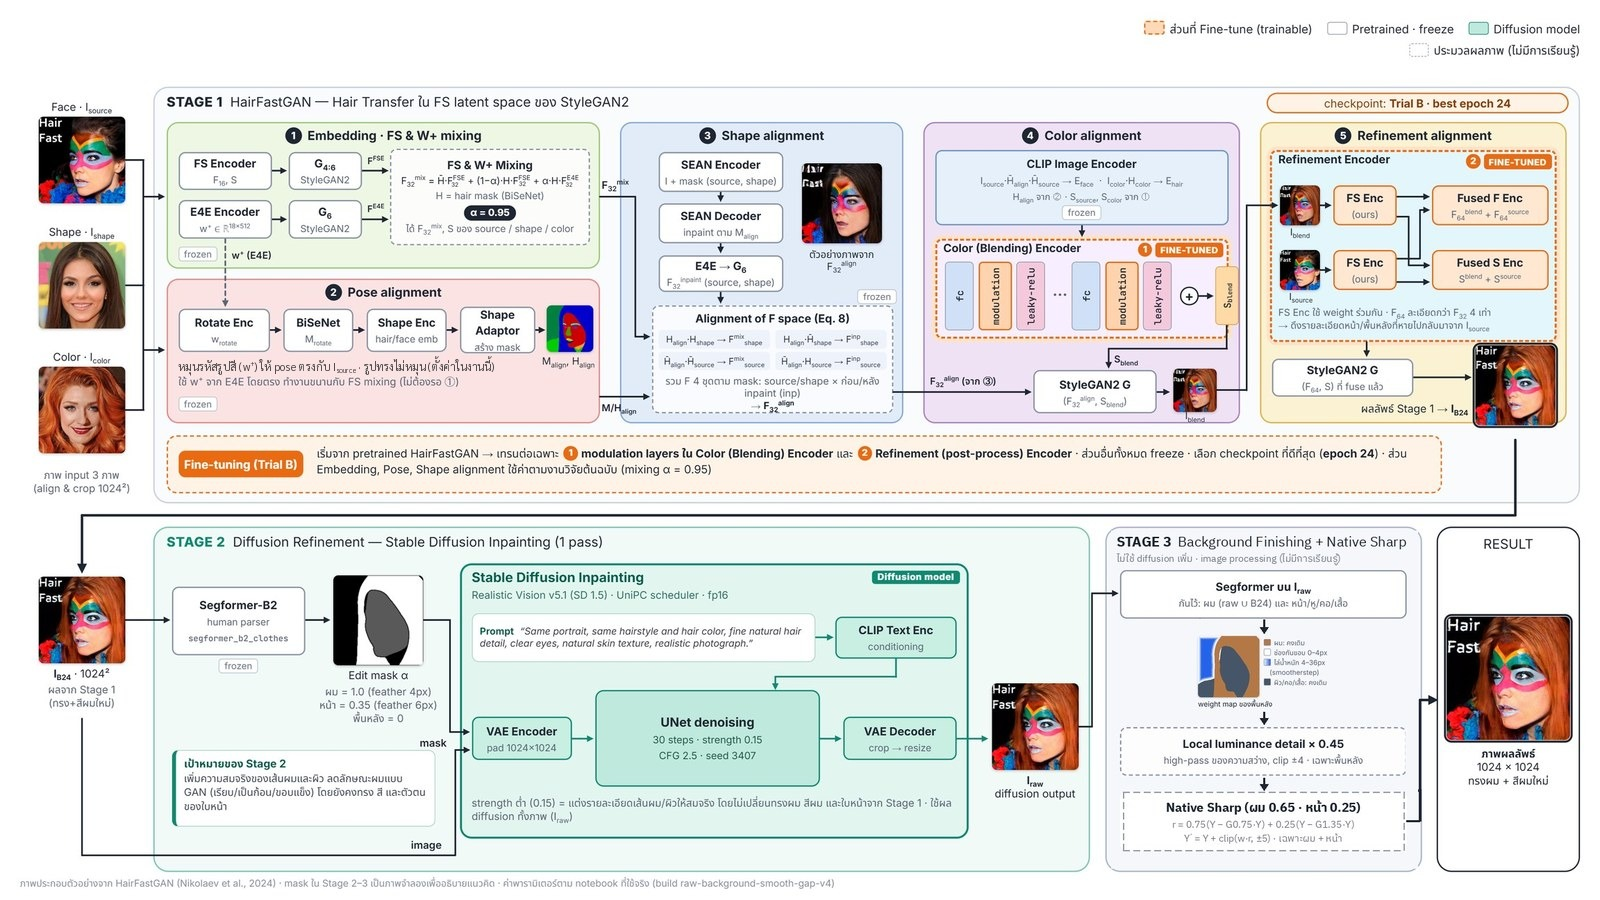
\includegraphics[width=\textwidth]{images/fig_pipeline_hfg_detail.jpg}
\caption{ขั้นตอนการทำงานของ HairFastGAN (ปรับจูน) + Stable Diffusion
แสดงโมดูลที่ล็อกไว้ โมดูลที่ปรับจูน และขั้นขัดเกลาที่เพิ่มเข้ามา}
\label{fig:pipe_hfg}
\par\vspace{3pt}{\footnotesize\raggedright หมายเหตุ: HFG = HairFastGAN, E4E = Encoder for Editing, SEAN = Semantic Region-Adaptive Normalization, CLIP = Contrastive Language-Image Pre-training, BiSeNet = Bilateral Segmentation Network, SegFormer = Segmentation Transformer\par}
\end{figure}

โมดูลแรก Embedding ทำหน้าที่เดียวกับขั้นที่ 1 ของ Barbershop แต่ใช้ FS Encoder และ E4E (Encoder for Editing)
คำนวณรหัส $F$ ($32 \times 32 \times 512$) และ $S$ (รหัสสไตล์ของชั้นถัดจาก $F$) ของทั้ง 3 ภาพในครั้งเดียว
เฉพาะบริเวณผมจะผสม $F$ จาก FS Encoder กับ $F$ จาก E4E ตามสมการที่~(\ref{eq:h_embed})
ซึ่งเป็นสมการที่~(\ref{eq:hfg_mix}) ในบทที่ 2 ที่เขียนให้สั้นลง
เหตุผลคือ $F$ จาก FS Encoder เก็บรายละเอียดของผมไว้แน่นจนเปลี่ยนสีผมได้ยาก
ส่วน $F$ จาก E4E หยาบกว่าแต่แก้ไขง่าย งานวิจัยนี้ใช้ค่าผสม 0.95 เท่ากับงานต้นฉบับ
คือบริเวณผมใช้ $F$ จาก E4E ร้อยละ 95 และจาก FS Encoder ร้อยละ 5 ส่วนใบหน้าและพื้นหลังใช้ FS Encoder ทั้งหมด
\begin{equation}
(F_{FS}, S) = E_{FS}(I), \qquad F_{hair} = 0.05 \cdot F_{FS} + 0.95 \cdot F_{E4E}
\label{eq:h_embed}
\end{equation}
\begin{vardef}
$E_{FS}$ & ตัวเข้ารหัส FS Encoder \\
$I$ & ภาพนำเข้า \\
$F_{hair}$ & แผนที่คุณลักษณะบริเวณผมที่ใช้ต่อ \\
$F_{FS}, F_{E4E}$ & แผนที่คุณลักษณะที่ได้จาก FS Encoder และจากการวาดรหัส $W^{+}$ ของ E4E ถึงชั้น $32 \times 32$
\end{vardef}

โมดูลที่สอง Pose ใช้ Rotate Encoder หมุนรหัสของภาพอ้างอิงให้หันตามใบหน้า
โดยแก้เฉพาะ 6 เวกเตอร์แรกของ $W^{+}$ ซึ่งควบคุมท่าทาง
แล้ววาดภาพที่หมุนแล้วส่งให้ BiSeNet หาหน้ากากผมที่หันถูกทาง ตามสมการที่~(\ref{eq:h_pose})
งานต้นฉบับหมุนทั้งภาพทรงผมและภาพสีผม แต่ในงานวิจัยนี้ผู้วิจัยปิดการหมุนของภาพทรงผม
และเปิดไว้เฉพาะภาพสีผม เพื่อหาหน้ากากผมของภาพสีผมสำหรับใช้ในโมดูล Color
เหตุผลคือภาพในชุดข้อมูลเป็นภาพหน้าตรงที่จัดตำแหน่งแล้ว จึงใช้หน้ากากของภาพทรงผมได้โดยตรง
และไม่เสี่ยงให้ทรงผมเพี้ยนจากการหมุน การตั้งค่านี้ใช้เหมือนกันทั้งตอนฝึก ตอนทดสอบ และบนเว็บ
\begin{equation}
w_{rotate} = \mathrm{RotateEnc}\left(w_{face}, w_{color}\right), \qquad
M_{rotate} = \mathrm{BiSeNet}\left(G(w_{rotate})\right)
\label{eq:h_pose}
\end{equation}
\begin{vardef}
$w_{face}, w_{color}$ & รหัส $W^{+}$ จาก E4E ของภาพใบหน้าและภาพสีผม \\
$w_{rotate}$ & รหัสของภาพสีผมที่หมุนให้หันตามใบหน้าแล้ว \\
$G$ & ตัวสร้างภาพ StyleGAN2 \\
$M_{rotate}$ & หน้ากากของภาพสีผมที่หมุนแล้ว
\end{vardef}

โมดูลที่สาม Shape ทำนายว่าทรงผมนี้เมื่ออยู่บนศีรษะของคนในภาพใบหน้าจะมีรูปร่างแบบใด
ได้เป็นหน้ากาก $M_{target}$ (ซึ่งคือ $M_\text{align}$ ในสมการที่~(\ref{eq:pose_mask}))
แล้วประกอบ $F$ ให้ผมไปอยู่ตามทรงนั้น โดยใช้ SEAN (Semantic Region-Adaptive Normalization) เติมส่วนที่ขาดหาย
ตามสมการที่~(\ref{eq:h_shape}) ซึ่งเป็นสมการที่~(\ref{eq:shape_combine}) ที่เขียนแบบย่อ
ผู้วิจัยใช้ $M_{target}$ นี้เป็นทรงเป้าหมายในการคำนวณค่าสูญเสียด้านทรงและค่า IoU (Intersection over Union) ของทั้งสองโมเดล
เพื่อให้ทั้งคู่ถูกวัดกับเป้าหมายเดียวกัน
\begin{equation}
M_{target} = \mathrm{Shape}\left(M_{face}, M_{shape}\right), \qquad
F_{align} = \mathrm{SEAN}\left(F_{face}, M_{target}\right)
\label{eq:h_shape}
\end{equation}
\begin{vardef}
$M_{face}$ & แผนที่ส่วนภาพของภาพใบหน้า \\
$M_{shape}$ & แผนที่ส่วนภาพของภาพทรงผม (ไม่หมุน) \\
$M_{target}$ & หน้ากากทรงผมเป้าหมายบนใบหน้านี้ \\
$F_{face}$ & แผนที่คุณลักษณะของภาพใบหน้า \\
$F_{align}$ & แผนที่คุณลักษณะที่มีทรงผมใหม่
\end{vardef}

โมดูลที่สี่ Color เป็นโมดูลแรกที่ผู้วิจัยปรับจูน และเป็นต้นเหตุของสีผมที่เป็นปื้น
CLIP อ่านสีผมจากภาพสีผมออกมาเป็นเวกเตอร์ แล้ว Blending Encoder ใช้เวกเตอร์นี้คำนวณค่าสเกลและค่าเลื่อน
ไปปรับ $S$ ทีละชั้น ได้ภาพกลาง $I_{pre}$ ซึ่งผมเป็นสีใหม่แล้ว ตามสมการที่~(\ref{eq:h_color})
ผู้วิจัยปรับเฉพาะชั้นปรับค่า (Modulation) ของ Blending Encoder ซึ่งเป็นจุดที่แปลงเวกเตอร์สีเป็นการเปลี่ยนแปลงของภาพ
\begin{equation}
S_{blend} = \mathrm{Blend}\left(S_{face}, S_{color}, e_{hair}, e_{face}\right), \qquad
I_{pre} = G\left(F_{align}, S_{blend}\right)
\label{eq:h_color}
\end{equation}
\begin{vardef}
$S_{face}, S_{color}$ & รหัสสไตล์ของภาพใบหน้าและภาพสีผม \\
$e_{hair}, e_{face}$ & เวกเตอร์จาก CLIP ของบริเวณผมในภาพสีผมและบริเวณใบหน้า \\
$S_{blend}$ & รหัสสไตล์ใหม่ \\
$I_{pre}$ & ภาพกลางที่ได้สีผมใหม่แต่ยังไม่ผ่าน Refinement
\end{vardef}

โมดูลที่ห้า Refinement เป็นโมดูลที่สองที่ปรับจูน และเป็นต้นเหตุของใบหน้าที่ซีด
ภาพ $I_{pre}$ ผ่านการเข้ารหัสที่ขนาด $32 \times 32$ มาแล้ว รายละเอียดของผิว ตา และฉากหลังจึงหายไปบางส่วน
โมดูลนี้ (ในโค้ดชื่อ PostProcess) ใช้ FS Encoder ตัวใหญ่แปลงทั้ง $I_{pre}$ และภาพใบหน้าเดิม
เป็นคุณลักษณะขนาด $64 \times 64$ ซึ่งละเอียดกว่า แล้วใช้ตัวผสม Fused $F$/$S$ รวมกัน ก่อนให้ StyleGAN2 วาดภาพ
เพื่อดึงผิว ตา และฉากหลังจากภาพจริงกลับมา โดยยังคงผมใหม่ไว้ ตามสมการที่~(\ref{eq:h_post})
ผู้วิจัยปรับจูนทั้งโมดูล
\begin{equation}
I_{final} = \mathrm{Post}\left(I_{pre}, I_{face}\right)
\label{eq:h_post}
\end{equation}
\begin{vardef}
$I_{final}$ & ภาพผลลัพธ์สุดท้ายของ HairFastGAN \\
$\mathrm{Post}$ & โมดูล PostProcess (FS Encoder ตัวใหญ่ ตัวผสม Fused $F$/$S$ และ StyleGAN2 ที่ล็อกไว้) ตามสมการที่~(\ref{eq:i_final}) \\
$I_{face}$ & ภาพใบหน้าต้นฉบับ
\end{vardef}

เหตุผลที่ปรับเพียงสองโมดูลนี้ คือปัญหาที่เห็นจากโมเดลตั้งต้นอยู่ที่สีและใบหน้า ไม่ได้อยู่ที่ทรง
อีกเหตุผลหนึ่งคือข้อมูล 150 ชุดน้อยเกินกว่าจะฝึกทั้งระบบ ถ้าปลดล็อกทุกโมดูล
โมเดลมีแนวโน้มจะจำชุดฝึกได้แต่ลืมสิ่งที่เคยเรียนจากข้อมูลจำนวนมากของผู้พัฒนา
ผลของสามโมดูลแรกที่ล็อกไว้จึงคำนวณเพียงครั้งเดียวแล้วเก็บไว้ใช้ตลอดการฝึก ซึ่งช่วยให้ฝึกได้เร็วขึ้นมาก
ภาพที่~\ref{fig:stage2_output} เปรียบเทียบผลของสองโมเดลจากภาพนำเข้าชุดเดียวกัน
ซ้ายคือ HairFastGAN และขวาคือ Barbershop ทั้งสองวางทรงและสีได้ใกล้ภาพอ้างอิง
แต่ถ้าดูใกล้ ๆ จะเห็นว่าเนื้อผมและสีผิวต่างกัน ซึ่งเป็นสิ่งที่การปรับจูนพยายามแก้

\begin{figure}[!htbp]
    \centering
    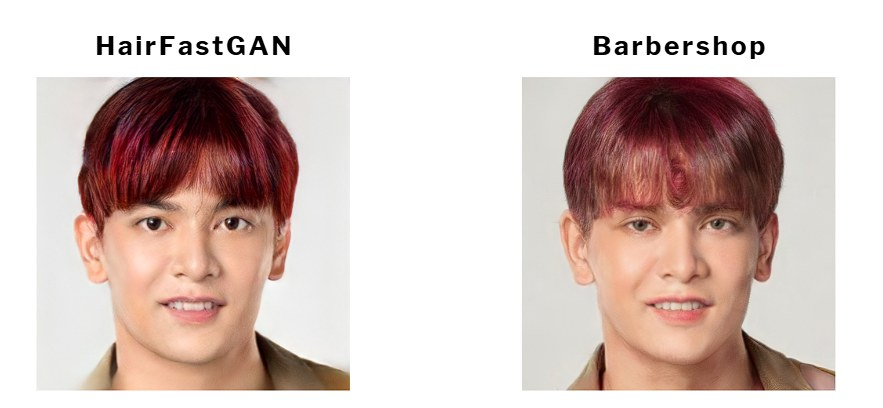
\includegraphics[width=0.7\textwidth]{images/stage2_output.jpg}
    \caption{ตัวอย่างภาพผลลัพธ์จาก HairFastGAN และ Barbershop จากภาพนำเข้าชุดเดียวกัน}
    \label{fig:stage2_output}
\end{figure}

% -----------------------------------------------------------
\section{การปรับจูนโมเดล}
% -----------------------------------------------------------

ทั้งสองโมเดลปรับจูนภายใต้เป้าหมายหลักชุดเดียวกัน แต่รายละเอียดต่างกันตามโครงสร้างของแต่ละโมเดล
และทุก Trial เริ่มจากน้ำหนักทางการชุดเดิม
ภาพที่~\ref{fig:finetune} แบ่งเป็นสองแถว แถวบนคือสิ่งที่เกิดกับข้อมูลหนึ่งตัวอย่าง
ข้อมูลผ่านส่วนที่ล็อกไว้ (กรอบน้ำเงิน) แล้วผ่านส่วนที่ฝึก (กรอบส้มเส้นประ) จนได้ภาพผลลัพธ์
จากนั้นคำนวณค่าสูญเสียรวม แล้วลูกศรย้อนกลับแสดงว่าเกรเดียนต์ถูกส่งกลับไปปรับเฉพาะส่วนที่ฝึก
ทำแบบนี้จนครบ 150 ตัวอย่าง นับเป็น 1 Epoch
แถวล่างคือสิ่งที่ทำหลังจบแต่ละ Epoch คือวัดผลบนชุดตรวจสอบ 9 ชุด คิดคะแนนเทียบกับ Epoch 0
ตรวจว่าผ่านเกณฑ์ทั้ง 5 ด่านหรือไม่ แล้วเก็บ Checkpoint ที่ดีที่สุดไว้

\begin{figure}[!htbp]
\centering
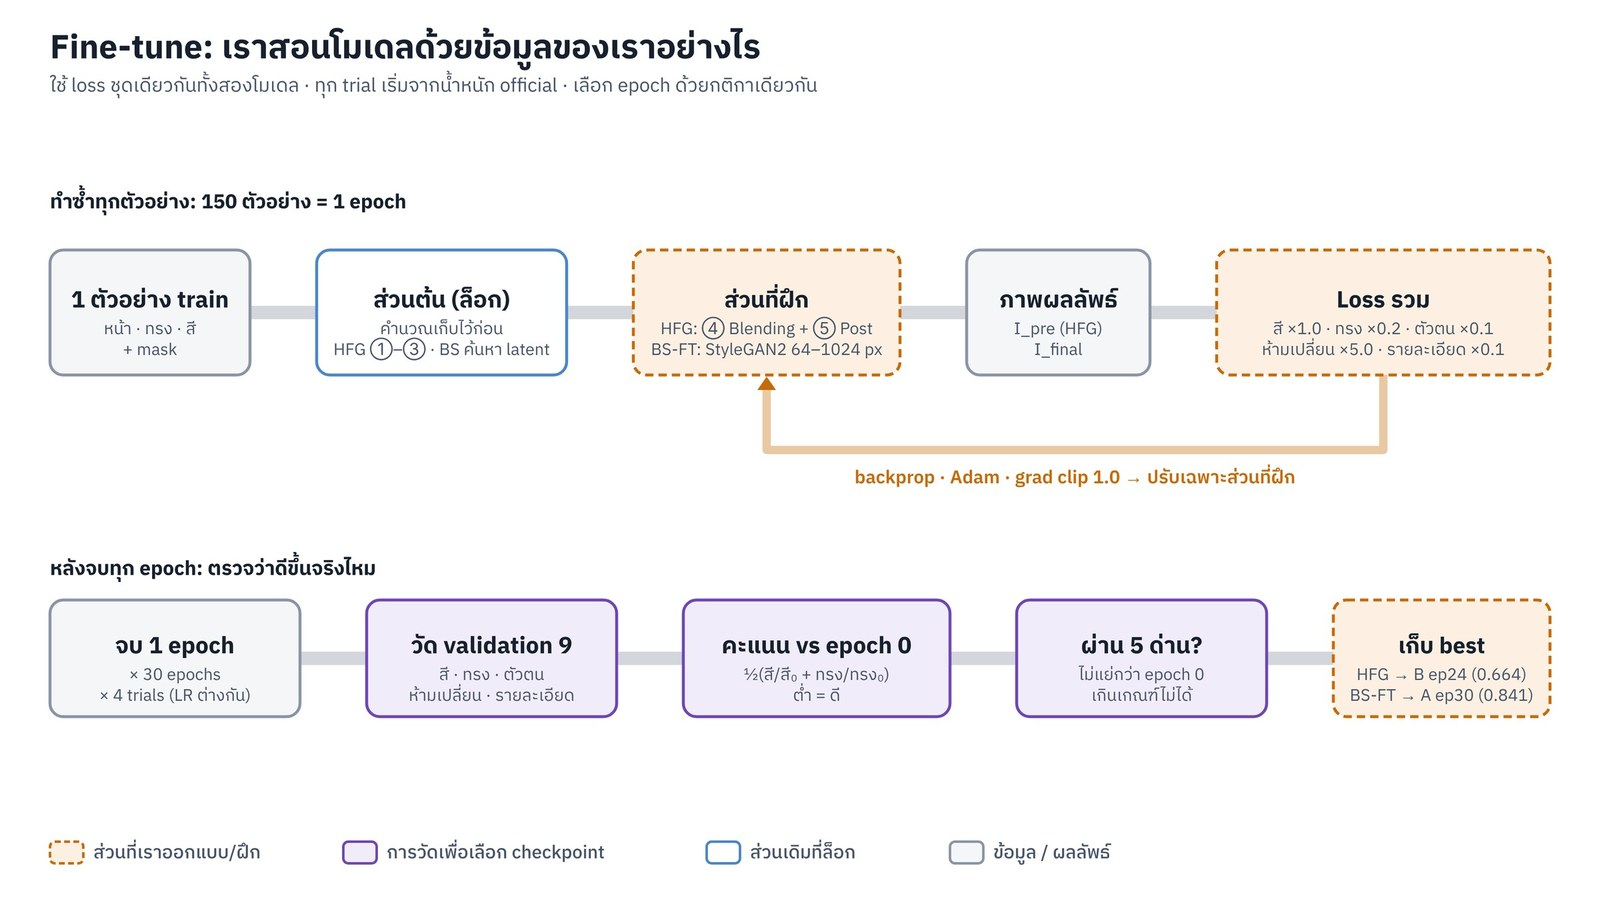
\includegraphics[width=\textwidth]{images/fig_finetune.jpg}
\caption{ขั้นตอนการปรับจูน: วนฝึกทุกตัวอย่างในชุดฝึก
และตรวจสอบบนชุดตรวจสอบหลังจบทุก Epoch}
\label{fig:finetune}
\par\vspace{3pt}{\footnotesize\raggedright หมายเหตุ: HFG = HairFastGAN, BS = Barbershop, BS-FT (Barbershop-FT) = Barbershop ที่ปรับจูนแล้ว (Fine-tuned), B24 = น้ำหนักของ Trial B Epoch 24, ep = Epoch, A30 = น้ำหนักของ Trial A Epoch 30, Adam = Adaptive Moment Estimation\par}
\end{figure}

\subsection{ฟังก์ชันความสูญเสีย}
\label{sec:loss}

ฟังก์ชันความสูญเสียเป็นส่วนที่ผู้วิจัยใช้เวลาออกแบบมากที่สุด
เพราะเป็นสิ่งที่บอกโมเดลว่าภาพที่ดีควรเป็นอย่างไร
ถ้าวัดแค่สี โมเดลอาจเปลี่ยนสีผิวหน้าไปด้วย ถ้าวัดแค่ใบหน้า โมเดลอาจไม่เปลี่ยนอะไรเลย
ผู้วิจัยจึงแยกสิ่งที่ต้องการออกเป็น 5 ด้าน แล้วรวมกันแบบถ่วงน้ำหนักตามสมการที่~(\ref{eq:loss})
ทุกด้านยิ่งต่ำยิ่งดี และคำนวณบนภาพผลลัพธ์สุดท้าย
\begin{equation}
L = 1.0\,L_{color} + 0.2\,L_{shape} + 0.1\,L_{id} + 5.0\,L_{protect} + 0.1\,L_{detail}
\label{eq:loss}
\end{equation}
\begin{vardef}
$L$ & ค่าสูญเสียรวม \\
$L_{color}$ & ค่าสูญเสียด้านสีผม (สมการที่~\ref{eq:l_color}) \\
$L_{shape}$ & ค่าสูญเสียด้านทรงผม (สมการที่~\ref{eq:l_shape}) \\
$L_{id}$ & ค่าสูญเสียด้านเอกลักษณ์ใบหน้า (สมการที่~\ref{eq:l_id}) \\
$L_{protect}$ & ค่าสูญเสียด้านบริเวณที่ต้องคงเดิม (สมการที่~\ref{eq:l_protect}) \\
$L_{detail}$ & ค่าสูญเสียด้านรายละเอียดเส้นผม (สมการที่~\ref{eq:l_detail}) \\
1.0, 0.2, 0.1, 5.0, 0.1 & น้ำหนักของแต่ละด้าน
\end{vardef}

ด้านแรกคือสีผม $L_{color}$ ผู้วิจัยแปลงภาพเป็นปริภูมิสี Lab
เพราะระยะห่างของค่าในปริภูมินี้ใกล้กับความต่างที่ตาคนเห็น แล้วเลือกเฉพาะพิกเซลผมด้านใน (ตัดขอบผมออก)
จากนั้นเทียบค่าเปอร์เซ็นไทล์ที่ 10 ถึง 90 ของผมในภาพผลลัพธ์กับผมในภาพสีผม ตามสมการที่~(\ref{eq:l_color})
ที่ไม่ใช้ค่าเฉลี่ยของสี เพราะค่าเฉลี่ยไม่บอกว่าสีไล่เฉดอย่างไร
ผมที่เป็นปื้นสีเดียวอาจมีค่าเฉลี่ยเท่ากับผมจริงที่มีทั้งส่วนสว่างและส่วนเงา
การเทียบหลายเปอร์เซ็นไทล์จึงบังคับให้การกระจายของสีตรงกันด้วย
และการตัดค่าที่ต่ำกว่าเปอร์เซ็นไทล์ที่ 10 และสูงกว่าเปอร์เซ็นไทล์ที่ 90 ออก ช่วยไม่ให้พิกเซลผิดปกติ เช่น แสงสะท้อน มีผลมากเกินไป
ข้อดีอีกข้อคือวิธีนี้ไม่ขึ้นกับตำแหน่งของผม จึงใช้ได้แม้ทรงผมของสองภาพจะต่างกัน
\begin{equation}
\begin{gathered}
E_L = \operatorname*{mean}_{p \in [10,90]} \left\lvert Q_p(L_{out}) - Q_p(L_{ref}) \right\rvert \\
E_{ab} = \text{ค่าเดียวกันเฉลี่ยรวมช่อง } a \text{ และ } b, \qquad
L_{color} = \frac{E_L + E_{ab}}{100}
\end{gathered}
\label{eq:l_color}
\end{equation}
\begin{vardef}
$E_L$ & ความคลาดเคลื่อนของความสว่างผม \\
$E_{ab}$ & ความคลาดเคลื่อนของสีผม (ช่อง $a$ และ $b$) \\
$Q_p(\cdot)$ & ค่าเปอร์เซ็นไทล์ที่ $p$ ของพิกเซลผม \\
$L_{out}, L_{ref}$ & ค่าความสว่างของผมในภาพผลลัพธ์และในภาพสีผม \\
$p$ & เปอร์เซ็นไทล์ 9 ค่า คือ 10, 20, \ldots, 90 \\
100 & ตัวหารเพื่อปรับสเกลให้อยู่ในช่วงเดียวกับค่าสูญเสียอื่น
\end{vardef}
ตัวชี้วัด ``สีผิด'' ที่รายงานในบทที่ 4 คือค่า $E_L + E_{ab}$ ก่อนหารด้วย 100
ยิ่งต่ำยิ่งแปลว่าสีผมใกล้กับภาพสีผม

ด้านที่สองคือทรงผม $L_{shape}$ ซึ่งดูว่าผมในภาพผลลัพธ์อยู่ตรงกับ $M_{target}$ หรือไม่
ผู้วิจัยใช้ค่าสองส่วนรวมกันตามสมการที่~(\ref{eq:l_shape})
ส่วนแรกคือครอสเอนโทรปีแบบสองค่า (Binary Cross-Entropy: BCE) แบบถ่วงดุล ซึ่งลงโทษทีละพิกเซล
โดยหาค่าเฉลี่ยในบริเวณผมและนอกบริเวณผมแยกกัน แล้วนำมาเฉลี่ยอีกครั้ง
เพราะ BCE แบบธรรมดาจะถูกพื้นหลังซึ่งมีจำนวนพิกเซลมากกว่าผมครอบงำ
ส่วนที่สองคือค่าสูญเสียไดซ์ (Dice Loss) ซึ่งดูการทับกันของผมทั้งก้อน
โดยบวก 1 ทั้งเศษและส่วนเพื่อกันการหารด้วยศูนย์
ส่วน Dice ไม่ขึ้นกับขนาดของผม คนผมสั้นและคนผมยาวจึงถูกวัดอย่างเท่าเทียม
\begin{equation}
\begin{aligned}
L_{shape} = &\ \frac{1}{2}\left(\frac{\sum y\,b}{\sum y} + \frac{\sum (1-y)\,b}{\sum (1-y)}\right)
+ 1 - \frac{2\sum p\,y + 1}{\sum p + \sum y + 1} \\
b = &-\left[ y\log p + (1-y)\log(1-p) \right]
\end{aligned}
\label{eq:l_shape}
\end{equation}
\begin{vardef}
$p$ & ความน่าจะเป็นที่พิกเซลเป็นผม ซึ่ง BiSeNet ทำนายจากภาพผลลัพธ์ \\
$y$ & ค่าของหน้ากากทรงเป้าหมาย $M_{target}$ (1 = ควรเป็นผม) \\
$b$ & ค่า BCE ของแต่ละพิกเซล \\
$\sum$ & ผลรวมทุกพิกเซลของภาพ
\end{vardef}

ด้านที่สามคือใบหน้ายังเป็นคนเดิมหรือไม่ $L_{id}$
ใช้ ArcFace แปลงใบหน้าในภาพผลลัพธ์และภาพต้นฉบับเป็นเวกเตอร์ แล้ววัดว่าสองเวกเตอร์ชี้ไปทางเดียวกันเพียงใด
ตามสมการที่~(\ref{eq:l_id}) ถ้าเป็นคนเดียวกัน ค่าจะใกล้ 0
\begin{equation}
L_{id} = 1 - \cos\left(\mathrm{ArcFace}(I_{out}), \mathrm{ArcFace}(I_{face})\right)
\label{eq:l_id}
\end{equation}
\begin{vardef}
$\mathrm{ArcFace}(\cdot)$ & เวกเตอร์ใบหน้า 512 มิติจาก ArcFace \\
$I_{out}, I_{face}$ & ภาพผลลัพธ์และภาพใบหน้าต้นฉบับ \\
$\cos$ & ความคล้ายโคไซน์ (1 = เหมือนที่สุด)
\end{vardef}

ด้านที่สี่คือบริเวณที่ต้องคงเดิม $L_{protect}$ ผู้วิจัยดูทุกพิกเซลที่ไม่ใช่ผมเดิมและไม่ใช่ผมใหม่
แล้วหาค่าเฉลี่ยว่าสี RGB (Red, Green, Blue) ต่างจากภาพต้นฉบับเท่าใด ตามสมการที่~(\ref{eq:l_protect})
ค่าถูกปรับให้อยู่ในช่วง 0--1 เช่น ค่า 0.04 หมายถึงต่างกันโดยเฉลี่ยประมาณ 10 จาก 255 ระดับ
ซึ่งเป็นความต่างที่ตาเริ่มสังเกตเห็น ด้านนี้ตรงกับปัญหาใบหน้าซีดของ HairFastGAN โดยตรง
\begin{equation}
\begin{gathered}
L_{protect} = \frac{1}{\lvert \Omega \rvert} \sum_{(x,y) \in \Omega}
\left\lvert I_{out}(x,y) - I_{face}(x,y) \right\rvert \\
\Omega = \text{นอก}\left(\text{ผมเดิม} \cup \text{ผมใหม่}\right)
\end{gathered}
\label{eq:l_protect}
\end{equation}
\begin{vardef}
$\Omega$ & เซตของพิกเซลนอกบริเวณผมเดิมและผมใหม่ \\
$\lvert \Omega \rvert$ & จำนวนพิกเซลในเซต $\Omega$ \\
$I_{out}(x,y), I_{face}(x,y)$ & ค่าสี RGB ของพิกเซล $(x,y)$ ในภาพผลลัพธ์และภาพต้นฉบับ
\end{vardef}

ด้านที่ห้าคือรายละเอียดของเส้นผม $L_{detail}$ ด้านนี้มีไว้กันทางลัดที่โมเดลอาจเลือก
คือเมื่อพยายามลด $L_{color}$ โมเดลอาจทำให้ผมเรียบเป็นปื้น
เพราะผมที่เรียบควบคุมสีได้ง่ายกว่าผมที่เห็นเป็นเส้น ซึ่งจะย้อนกลับไปเป็นปัญหาเดิมที่ต้องการแก้
$L_{detail}$ จึงวัดค่า MAE (Mean Absolute Error) ของรายละเอียดบริเวณผมเทียบกับภาพอ้างอิง เพื่อกันไม่ให้เนื้อผมหายไป
สำหรับ HairFastGAN ภาพอ้างอิงคือภาพกลาง $I_{pre}$
ซึ่งยังไม่ผ่านโมดูล Refinement และมีรายละเอียดผมต่างจากภาพผลลัพธ์อยู่แล้วตั้งแต่ก่อนฝึก
ค่านี้จึงไม่เป็น 0 ตั้งแต่ Epoch 0 (0.5816 ในตารางที่~\ref{tab:loss_example})
ส่วน Barbershop-FT ภาพอ้างอิงคือภาพของ Barbershop ก่อนปรับจูน
ซึ่งเป็นภาพเดียวกับผลลัพธ์ที่ Epoch 0 ค่านี้จึงเริ่มจาก 0
คำว่า ``รายละเอียด'' ในที่นี้คือความสว่างที่ลบค่าเฉลี่ยของพิกเซลรอบข้าง แล้วหารด้วยส่วนเบี่ยงเบนมาตรฐานของพิกเซลรอบข้าง
จึงเหลือแต่ลายเส้นผมโดยไม่ขึ้นกับว่าผมสีอ่อนหรือเข้ม
และคำนวณเฉพาะผมด้านในที่หดขอบเข้ามา 4 พิกเซล ที่ความละเอียด 256 และ 512 พิกเซล แล้วเฉลี่ยสองค่า
ตามสมการที่~(\ref{eq:l_detail})
\begin{equation}
\begin{gathered}
\mathcal{T}(I) = \frac{Y - \mu_{9}(Y)}{\sqrt{\sigma^2_{9}(Y) + 0.001}}, \qquad
L_{detail} = \frac{1}{2} \sum_{r \in \{256, 512\}}
\frac{1}{\lvert \Omega_r \rvert} \sum_{(x,y) \in \Omega_r}
\left\lvert \mathcal{T}(I^{r}_{out}) - \mathcal{T}(I^{r}_{ref}) \right\rvert
\end{gathered}
\label{eq:l_detail}
\end{equation}
\begin{vardef}
$\mathcal{T}(I)$ & รายละเอียดเฉพาะที่ของภาพ $I$ \\
$Y$ & ความสว่าง คือค่าเฉลี่ยของสามช่องสี RGB \\
$\mu_{9}, \sigma^2_{9}$ & ค่าเฉลี่ยและความแปรปรวนในหน้าต่าง $9 \times 9$ พิกเซลรอบแต่ละจุด \\
0.001 & ค่าคงที่กันการหารด้วยศูนย์ในบริเวณที่เรียบ \\
$r$ & ความละเอียดที่ย่อภาพลงไปคำนวณ \\
$I^{r}_{out}, I^{r}_{ref}$ & ภาพผลลัพธ์และภาพอ้างอิงที่ย่อเป็นขนาด $r \times r$ \\
$\Omega_r$ & พิกเซลผมด้านในที่ขนาด $r$ (หน้ากากผมที่หดขอบเข้ามา 4 พิกเซล)
\end{vardef}

น้ำหนักที่คูณแต่ละด้านไม่ได้ตั้งตามความสำคัญ แต่ตั้งเพื่อให้แต่ละด้านมีผลต่อการฝึกใกล้เคียงกัน
เพราะค่าดิบของแต่ละด้านมีขนาดต่างกันมาก เช่น $L_{protect}$ มีค่าเพียงประมาณ 0.04
ถ้าคูณ 1 ก็แทบไม่มีผล จึงคูณ 5.0 ให้มีขนาดประมาณ 0.19
ขณะที่ $L_{shape}$ มีค่าประมาณ 0.46 แต่ขยับได้น้อยเพราะส่วนที่ควบคุมทรงถูกล็อกไว้เกือบทั้งหมด จึงคูณเพียง 0.2
สำหรับ HairFastGAN ผู้วิจัยเพิ่มค่าสูญเสียอีกสองส่วน ซึ่งในเล่มนี้เรียกรวมว่าค่าสูญเสียส่วนเพิ่ม ตามสมการที่~(\ref{eq:loss_hfg})
ส่วนแรกคือวัดสีและทรงที่ภาพกลาง $I_{pre}$ ด้วย (Deep Supervision)
เพราะถ้าวัดแค่ภาพสุดท้าย สัญญาณที่ส่งกลับไปถึง Blending Encoder ต้องผ่าน Refinement ก่อน ทำให้เรียนรู้ได้ช้า
ส่วนที่สองคือค่าสูญเสียยึดรหัส (Latent Anchor) ที่กันไม่ให้รหัสลอยห่างจากค่าเดิมมากเกินไป
Barbershop-FT ไม่มีสองส่วนนี้ เพราะไม่มีภาพกลางที่ฝึกได้
\begin{equation}
L_{HFG} = L + 0.5\,L_{color}(I_{pre}) + 0.1\,L_{shape}(I_{pre}) + 0.01\,\mathrm{MSE}(z, z_0)
\label{eq:loss_hfg}
\end{equation}
\begin{vardef}
$L_{HFG}$ & ค่าสูญเสียรวมของ HairFastGAN \\
$L_{color}(I_{pre}), L_{shape}(I_{pre})$ & ค่าสูญเสียด้านสีและทรงที่คำนวณบนภาพกลาง $I_{pre}$ \\
$\mathrm{MSE}(z, z_0)$ & ค่าความผิดพลาดกำลังสองเฉลี่ยระหว่างรหัสปัจจุบัน $z$ กับรหัสเริ่มต้น $z_0$
\end{vardef}

\subsection{ขั้นตอนการฝึกและการตั้งค่า}

การปรับน้ำหนักหนึ่งครั้ง (1 Update) มีลำดับดังนี้ เริ่มจากรันโมเดลไปข้างหน้าจากรหัสที่เก็บไว้จนได้ภาพ
คำนวณ $L$ ตามสมการที่~(\ref{eq:loss}) แล้วหาอนุพันธ์ $\partial L / \partial \theta$ ย้อนกลับ
ผ่าน ArcFace, BiSeNet และตัวสร้างภาพมาจนถึง $\theta$
(ส่วนที่ล็อกไว้ยังส่งเกรเดียนต์ผ่านได้ เพียงแต่น้ำหนักของส่วนนั้นไม่ถูกปรับ)
จากนั้นปรับ $\theta$ ด้วย Adam (Adaptive Moment Estimation) ($\beta_1 = 0.9$, $\beta_2 = 0.999$) ตามสมการที่~(\ref{eq:adam})
ก่อนปรับจะย่อขนาดของเกรเดียนต์ไม่ให้เกิน 1.0 (Gradient Clipping) ตามสมการที่~(\ref{eq:clip})
เพราะในข้อมูลมีบางชุดที่ยากมาก เช่น ทรงผมกับใบหน้าต่างกันมาก
ชุดแบบนี้ให้เกรเดียนต์ใหญ่ผิดปกติ และอาจผลักโมเดลไปไกลในการปรับครั้งเดียว
\begin{equation}
g \leftarrow g \cdot \min\left(1, \frac{1.0}{\lVert g \rVert}\right)
\label{eq:clip}
\end{equation}
\begin{vardef}
$g$ & เวกเตอร์เกรเดียนต์ของพารามิเตอร์ทั้งหมดที่ฝึก \\
$\lVert g \rVert$ & ขนาด (Norm) ของเวกเตอร์เกรเดียนต์ \\
1.0 & ขนาดสูงสุดที่อนุญาต
\end{vardef}

การฝึกใช้ขนาดชุดย่อย (Batch Size) เท่ากับ 1 เพราะภาพขนาด $1024 \times 1024$ ใช้หน่วยความจำมาก
รวมเป็น 150 ตัวอย่าง $\times$ 30 Epoch = 4,500 Updates ต่อ Trial
ผู้วิจัยไม่ทราบล่วงหน้าว่าอัตราการเรียนรู้เท่าใดเหมาะสม จึงทดลอง 2 ค่าสำหรับพารามิเตอร์แต่ละกลุ่ม
รวม $2 \times 2 = 4$ Trial ดังตารางที่~\ref{tab:trials}
คอลัมน์ ``กลุ่มแรก'' คือส่วนหลักที่ทำงานเรื่องสี (Barbershop: ชั้นคอนโวลูชัน 64--1024 พิกเซล;
HairFastGAN: Blending Encoder) ส่วนคอลัมน์ ``กลุ่มหลัง'' คือส่วนที่อยู่ใกล้ภาพผลลัพธ์
(Barbershop: ชั้น ToRGB; HairFastGAN: PostProcess)
กลุ่มหลังตั้งค่าให้ต่ำกว่า เพราะขยับเพียงเล็กน้อยก็เปลี่ยนภาพทั้งภาพ
ตัวเลขในวงเล็บคือค่าเดียวกันที่เขียนเป็นทศนิยม จะเห็นว่าทุกค่าต่ำมาก
ซึ่งตั้งใจให้เป็นเช่นนั้น เพราะต้องการ ``ขยับ'' โมเดลที่ดีอยู่แล้วทีละน้อย ไม่ใช่สอนใหม่ทั้งหมด
ทุก Trial ใช้ Seed ข้อมูล ฟังก์ชันความสูญเสีย และจำนวน Update เท่ากัน
ผลที่ต่างกันจึงมาจากอัตราการเรียนรู้เพียงอย่างเดียว

\begin{table}[!htbp]
\centering
\caption{อัตราการเรียนรู้ของ 4 Trial}
\label{tab:trials}
\begin{tabular}{|c|c|c|}
\hline
\textbf{Trial} & \textbf{\shortstack{กลุ่มแรก\\(BS: Synthesis · HFG: Blending)}} & \textbf{\shortstack{กลุ่มหลัง\\(BS: ToRGB · HFG: PostProcess)}} \\ \hline
A & $1 \times 10^{-5}$ (0.00001) & $1 \times 10^{-6}$ (0.000001) \\ \hline
B & $1 \times 10^{-5}$ (0.00001) & $5 \times 10^{-7}$ (0.0000005) \\ \hline
C & $5 \times 10^{-6}$ (0.000005) & $1 \times 10^{-6}$ (0.000001) \\ \hline
D & $5 \times 10^{-6}$ (0.000005) & $5 \times 10^{-7}$ (0.0000005) \\ \hline
\end{tabular}
\par\vspace{3pt}{\footnotesize\raggedright หมายเหตุ: BS = Barbershop, HFG = HairFastGAN\par}

\end{table}

% -----------------------------------------------------------
\section{การเลือก Checkpoint}
\label{sec:select}
% -----------------------------------------------------------

4 Trial $\times$ 30 Epoch $\times$ 2 โมเดล ทำให้มีผลการตรวจสอบราย Epoch รวม 240 จุด
แต่จำนวนจุดที่ประเมินไม่เท่ากับจำนวนไฟล์น้ำหนักที่บันทึกไว้
HairFastGAN เลือกน้ำหนักได้จากทุก Epoch ขณะที่ Barbershop-FT มีไฟล์น้ำหนักเฉพาะ Epoch 0 และ 30
จึงเลือกโมเดลหลังปรับจูนได้เฉพาะ Epoch 30 ของแต่ละ Trial ขอบเขตการเลือกของสองโมเดลจึงไม่เท่ากัน
ถ้าเลือกด้วยการเปิดดูภาพทีละตัว ผลจะขึ้นกับความรู้สึก และถ้าเลือกซ้ำอาจได้คนละตัว
ผู้วิจัยจึงกำหนดสูตรคะแนนและเกณฑ์คัดเลือกไว้ โดยมีการแก้ไขเกณฑ์ด้านรายละเอียดผมภายหลัง ตามที่อธิบายไว้ด้านล่าง
และใช้เกณฑ์ฉบับแก้ไขกับทั้งสองโมเดล
ทุกครั้งที่จบ Epoch จะวัดผลบนชุดตรวจสอบ 9 ชุด และเทียบกับ Epoch 0 ของ Trial เดียวกันเสมอ
คะแนนบนชุดทดสอบของ Checkpoint หลังปรับจูนไม่ถูกนำมาใช้จัดอันดับในขั้นนี้
ส่วนการที่เคยดูผลของโมเดลก่อนปรับจูน (Baseline) บนชุดทดสอบและการแก้เกณฑ์ อธิบายไว้ด้านล่าง
กติกามี 3 ขั้น ดังนี้

ขั้นที่ 1 คือคิดคะแนน (ยิ่งต่ำยิ่งดี) จากความผิดพลาดของสีและทรง ตามสมการที่~(\ref{eq:score})
ปัญหาคือสีผิดมีหน่วยเป็นระดับสี Lab (ค่าประมาณ 14) ส่วนทรงผิดเป็นสัดส่วน (ค่าประมาณ 0.1)
ถ้าบวกกันตรง ๆ สีจะกลบทรงจนหมด ผู้วิจัยจึงหารแต่ละค่าด้วยค่าที่ Epoch 0 ก่อน
ทำให้ทั้งสองค่ากลายเป็น ``สัดส่วนเทียบกับตอนเริ่ม'' แล้วจึงหาค่าเฉลี่ย
Epoch 0 จึงได้คะแนน 1.00 เสมอ และคะแนน 0.66 หมายถึงความผิดพลาดเหลือร้อยละ 66 ของตอนก่อนฝึก
\begin{equation}
\text{score} = \frac{1}{2}\left( \frac{c}{c_0} + \frac{e}{e_0} \right), \qquad e = 1 - \mathrm{IoU}
\label{eq:score}
\end{equation}
\begin{vardef}
$c$ & สีผิด ($E_L + E_{ab}$) เฉลี่ยบนชุดตรวจสอบ ณ Epoch ที่พิจารณา \\
$e$ & ทรงผิด เท่ากับ $1 - \mathrm{IoU}$ \\
$c_0, e_0$ & ค่า $c$ และ $e$ ที่ Epoch 0 ของ Trial เดียวกัน
\end{vardef}

ขั้นที่ 2 คือตรวจเกณฑ์ขั้นต่ำ 5 ข้อ ซึ่งในเล่มนี้เรียกว่า ``ด่าน'' ตามตารางที่~\ref{tab:gates}
คะแนนในขั้นที่ 1 ดูเพียงสีกับทรง โมเดลจึงอาจได้คะแนนดีทั้งที่ใบหน้าหรือพื้นหลังเพี้ยน
ด่านมีไว้จับกรณีแบบนี้ แต่ละแถวในตารางคือตัวชี้วัดหนึ่งด้าน
และคอลัมน์ ``ผ่านเมื่อ'' คือขอบเขตที่ยอมรับได้เมื่อเทียบกับ Epoch 0
สองด่านแรก (สีและทรง) ต้องไม่แย่กว่าตอนเริ่มเลย เพราะเป็นเป้าหมายหลักของการปรับจูน
ส่วนอีกสามด่านยอมให้แย่ลงได้เล็กน้อยตามขอบที่กำหนด เพราะการแก้สีย่อมกระทบส่วนอื่นบ้าง
Checkpoint ที่ไม่ผ่านแม้เพียงด่านเดียวจะไม่ถูกนำมาพิจารณา

\begin{table}[!htbp]
\centering
\caption{ด่านที่ Checkpoint ต้องผ่าน (เทียบกับ Epoch 0)}
\label{tab:gates}
\begin{tabular}{|c|L{5.4cm}|L{5.4cm}|}
\hline
\textbf{ด่าน} & \textbf{ตัวชี้วัด} & \textbf{ผ่านเมื่อ} \\ \hline
1 & สีผิด ($E_L + E_{ab}$) & ไม่มากกว่า Epoch 0 \\ \hline
2 & IoU ทรงผม & ไม่น้อยกว่า Epoch 0 \\ \hline
3 & เอกลักษณ์ใบหน้า (ArcFace) & ลดลงได้ไม่เกิน 0.02 \\ \hline
4 & บริเวณที่ต้องคงเดิม (MAE) & เพิ่มขึ้นได้ไม่เกิน 0.01 \\ \hline
5 & รายละเอียดผม (Detail MAE) & เพิ่มขึ้นได้ไม่เกิน 0.091 \\ \hline
\end{tabular}
\par\vspace{3pt}{\footnotesize\raggedright หมายเหตุ: $E_L$, $E_{ab}$ = ความคลาดเคลื่อนของความสว่างและของสีผมในปริภูมิสี Lab, IoU = Intersection over Union (สัดส่วนพื้นที่ผมที่ทับกัน), ArcFace = โมเดลจดจำใบหน้าที่ใช้วัดความเหมือนของใบหน้า, MAE = Mean Absolute Error (ค่าความคลาดเคลื่อนสัมบูรณ์เฉลี่ย)\par}

\end{table}

ขั้นที่ 3 คือการเลือก สำหรับ HairFastGAN ให้เลือก Epoch ที่ผ่านครบ 5 ด่านและมีคะแนนต่ำสุดในแต่ละ Trial
ส่วน Barbershop-FT ตรวจเฉพาะน้ำหนัก Epoch 30 ที่บันทึกไว้ หากไม่ผ่านให้ใช้โมเดลก่อนปรับจูนต่อไป
ถ้าไม่มี Epoch ใดผ่านเลยให้ถือว่า Epoch 0 ชนะ จากนั้นเทียบ Trial A--D แล้วเลือกตัวที่คะแนนต่ำสุด

ด่านที่ 5 มีเรื่องที่ผู้วิจัยต้องบันทึกไว้อย่างตรงไปตรงมา ขอบของด่านนี้คือ $0.091 \approx 0.15 \times 0.6086$
หรือร้อยละ 15 ของค่ารายละเอียดผมของ HairFastGAN ที่ Epoch 0 และใช้กับทั้งสองโมเดล
แต่ในตอนแรก Barbershop-FT ใช้ขอบ 0.02 ซึ่งผู้วิจัยพบภายหลังว่าไม่เป็นธรรม
เพราะ Barbershop-FT เทียบรายละเอียดกับตัวเองก่อนปรับจูน ค่าเริ่มต้นจึงเป็น 0
และขยับเพียงเล็กน้อยก็ตกด่าน ขณะที่ HairFastGAN มีช่องให้ขยับมากกว่า
ผู้วิจัยจึงบันทึกการแก้ไขกติกา (Protocol Amendment) และใช้ขอบ 0.091 กับทั้งสองโมเดล
โดยแก้ก่อนประเมิน Checkpoint ใด ๆ บนชุดทดสอบ และไม่เปลี่ยนสูตรคะแนนหรือด่านอื่น
อย่างไรก็ตาม ผู้วิจัยขอเปิดเผยว่าก่อนแก้ไข เคยดูผลทดสอบของโมเดลก่อนปรับจูนมาแล้ว
แต่ Checkpoint ที่ถูกเลือกยังไม่เคยถูกวัดบนชุดทดสอบเลย

% -----------------------------------------------------------
\section{การทดสอบและตัวชี้วัด}
% -----------------------------------------------------------

เมื่อเลือก Checkpoint ได้แล้ว ผู้วิจัยล็อกไว้และวัดผลบนชุดทดสอบ 10 ชุดเพียงครั้งเดียว
เทียบกับโมเดลก่อนปรับจูน ด้วยตัวชี้วัดชุดเดียวกับที่ใช้เลือก และจับเวลาต่อภาพบน GPU A100
ตารางที่~\ref{tab:metrics} สรุปตัวชี้วัดทั้ง 5 ด้าน ซึ่งจับคู่กับ 5 ด้านของฟังก์ชันความสูญเสีย
คอลัมน์ ``ความหมาย'' บอกว่าตัวชี้วัดนั้นตอบคำถามอะไร
และคอลัมน์ ``ทิศทาง'' บอกว่าค่าแบบใดดี เช่น สีผิดและ MAE ยิ่งต่ำยิ่งดี
ส่วน IoU, ArcFace และ SSIM (Structural Similarity Index) ยิ่งสูงยิ่งดี
ด้านที่ 4 ใช้สองตัวชี้วัด เพราะ MAE บอกว่าสีเพี้ยนไปเท่าใด
ส่วน SSIM บอกว่าโครงสร้าง เช่น ขอบและลวดลาย ยังอยู่ครบหรือไม่

\begin{table}[!htbp]
\centering
\caption{ตัวชี้วัด 5 ด้านที่ใช้ทั้งการเลือก Checkpoint และการทดสอบ}
\label{tab:metrics}
\begin{tabular}{|c|L{3.0cm}|L{6.2cm}|L{2.6cm}|}
\hline
\textbf{ด้าน} & \textbf{ตัวชี้วัด} & \textbf{ความหมาย} & \textbf{ทิศทาง} \\ \hline
1 & สีผิด $E_L + E_{ab}$ & ความต่างสีผมกับผมในภาพสีผม (Lab ช่วงเปอร์เซ็นไทล์ 10--90) & ต่ำ = ดี \\ \hline
2 & IoU & พื้นที่ผมที่ทับกับทรงเป้าหมาย หารด้วยพื้นที่รวม & สูง = ดี \\ \hline
3 & ArcFace Cosine & ความเหมือนของใบหน้ากับภาพใบหน้านำเข้า & สูง = ดี \\ \hline
4 & MAE, SSIM & การเปลี่ยนแปลงของใบหน้า เสื้อผ้า และพื้นหลังนอกบริเวณผม & MAE ต่ำ, SSIM สูง \\ \hline
5 & Detail MAE & ความคมของเส้นผมเทียบภาพอ้างอิง (ใช้เป็นด่าน) & ไม่เพิ่มเกินเกณฑ์ \\ \hline
\end{tabular}
\par\vspace{3pt}{\footnotesize\raggedright หมายเหตุ: $E_L$, $E_{ab}$ = ความคลาดเคลื่อนของความสว่างและของสีผมในปริภูมิสี Lab, IoU = Intersection over Union (สัดส่วนพื้นที่ผมที่ทับกัน), ArcFace = โมเดลจดจำใบหน้าที่ใช้วัดความเหมือนของใบหน้า, MAE = Mean Absolute Error (ค่าความคลาดเคลื่อนสัมบูรณ์เฉลี่ย), SSIM = Structural Similarity Index (ดัชนีความคล้ายเชิงโครงสร้าง)\par}

\end{table}

ชุดทดสอบมีเพียง 10 ภาพ ค่าเฉลี่ยจึงแกว่งได้ง่าย
ถ้าภาพหนึ่งดีขึ้นมากผิดปกติ ค่าเฉลี่ยก็ดูดีขึ้นทั้งที่ภาพอื่นไม่เปลี่ยน
ผู้วิจัยจึงไม่ดูเฉพาะค่าเฉลี่ย แต่คำนวณผลต่างแบบจับคู่ทีละภาพ (ภาพเดียวกัน ค่าหลังปรับจูนลบค่าก่อนปรับจูน)
แล้วหาช่วงความเชื่อมั่น 95\% ด้วยวิธีบูตสแตรป โดยสุ่มเลือก 10 ภาพแบบใส่คืน 10,000 ครั้ง
ตามสมการที่~(\ref{eq:boot}) ถ้าช่วงที่ได้ไม่ครอบคลุมเลข 0
ก็กล่าวได้ว่าการเปลี่ยนแปลงนั้นไม่น่าเกิดจากความบังเอิญ
\begin{equation}
\bar d = \frac{1}{10}\sum_{i=1}^{10} d_i, \qquad
\mathrm{CI}_{95} = \left[ Q_{2.5}(\bar d^{*}),\; Q_{97.5}(\bar d^{*}) \right]
\label{eq:boot}
\end{equation}
\begin{vardef}
$d_i$ & ผลต่างของภาพทดสอบที่ $i$ เท่ากับค่าของโมเดลหลังปรับจูนลบค่าของโมเดลเดียวกันก่อนปรับจูน (เช่น BS-FT ลบ BS) \\
$\bar d$ & ค่าเฉลี่ยผลต่างของ 10 ภาพ \\
$\bar d^{*}$ & ค่าเฉลี่ยผลต่างที่ได้จากการสุ่มซ้ำแต่ละครั้ง (10,000 ค่า) \\
$Q_{2.5}, Q_{97.5}$ & เปอร์เซ็นไทล์ที่ 2.5 และ 97.5 ของค่า $\bar d^{*}$ \\
$\mathrm{CI}_{95}$ & ช่วงความเชื่อมั่น 95\%
\end{vardef}
ผู้วิจัยไม่ได้ใช้ FID (Fréchet Inception Distance) ซึ่งงานอื่นนิยมใช้
เพราะ FID ต้องใช้ภาพหลายพันภาพจึงจะให้ค่าที่นิ่ง ถ้าคำนวณจาก 10 ภาพ ตัวเลขจะไม่มีความหมาย

% -----------------------------------------------------------
\section{ขั้นขัดเกลาด้วย Diffusion}
\label{sec:diffusion}
% -----------------------------------------------------------

แม้ปรับจูนแล้ว ผมที่ได้จาก GAN ก็ยังดูนุ่มและเบลอ ไม่เห็นเป็นเส้นเหมือนภาพถ่าย
ผู้วิจัยจึงเพิ่มขั้นขัดเกลาด้วย Diffusion โดยตั้งใจให้ทำงาน ``เบา'' ที่สุดเท่าที่ยังได้ผล
GAN ยังเป็นตัวกำหนดทรงและสี ส่วน Diffusion มีหน้าที่เพียงเติมพื้นผิวของเส้นผมและผิวหน้า
และถูกจำกัดด้วยหน้ากากให้แก้ได้เฉพาะผมกับใบหน้า ขั้นนี้ไม่มีการฝึกเพิ่ม และใช้เวลารวมประมาณ 3.2 วินาทีต่อภาพ
ภาพที่~\ref{fig:diff_rows} แถวบนแสดงขั้นย่อย 4 ขั้นเรียงจากซ้ายไปขวา พร้อมสูตรและเวลาของแต่ละขั้น
ส่วนแถวล่างเป็นสรุปการปรับจูน HairFastGAN ที่อธิบายไปแล้ว ใส่ไว้เพื่อให้เห็นว่าสองส่วนต่อกันอย่างไร
เวลาที่เขียนในภาพเป็นของชุดภาพตัวอย่างหนึ่งชุด ส่วนเวลาในย่อหน้าต่อไปเป็นค่าเฉลี่ยของ HairFastGAN จาก 8 ชุดภาพในบทที่ 4

\begin{figure}[!htbp]
\centering
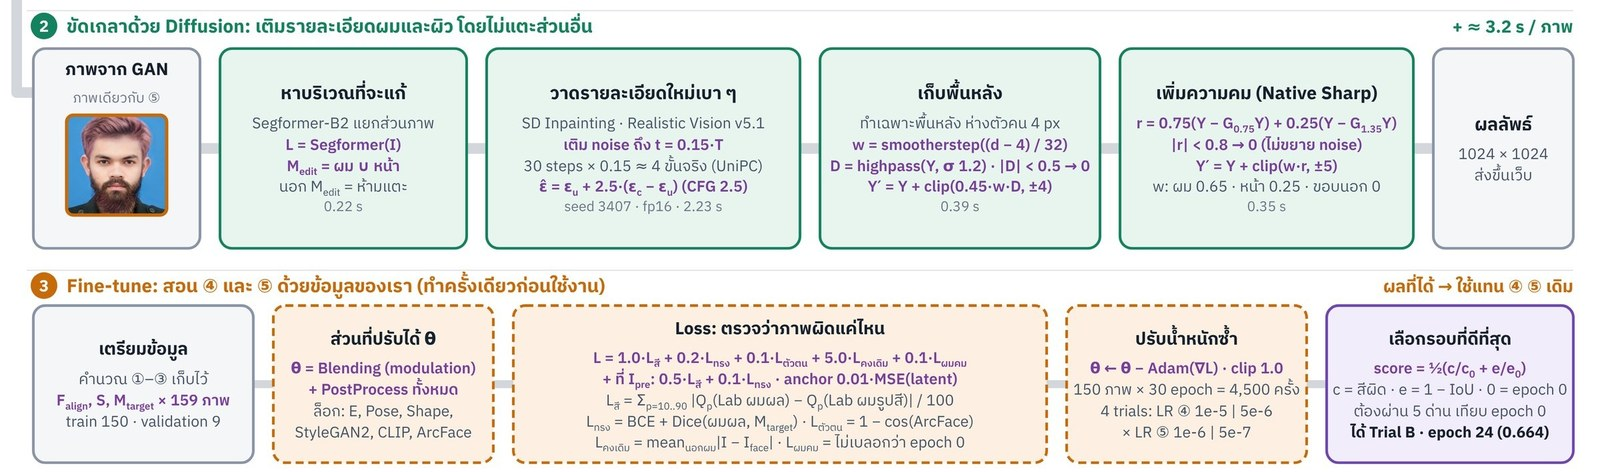
\includegraphics[width=\textwidth]{images/fig_diff_finetune_rows.jpg}
\caption{ขั้นขัดเกลาด้วย Diffusion (แถวบน) และสรุปการปรับจูน HairFastGAN (แถวล่าง)}
\label{fig:diff_rows}
\par\vspace{3pt}{\footnotesize\raggedright หมายเหตุ: HFG = HairFastGAN, SegFormer = Segmentation Transformer, UniPC = Unified Predictor-Corrector, CFG = Classifier-Free Guidance\par}
\end{figure}

ขั้นย่อยที่ 1 คือกำหนดบริเวณที่จะแก้ไข (0.23 วินาที)
SegFormer-B2 แบ่งส่วนของภาพจาก GAN แล้วรวมบริเวณผมกับใบหน้าเป็น $M_{edit}$ ตามสมการที่~(\ref{eq:m_edit})
เสื้อผ้าและพื้นหลังที่อยู่นอก $M_{edit}$ จะไม่ถูกวาดใหม่
แต่ยังต้องผ่านการบีบอัดและคืนสภาพของ VAE (Variational Autoencoder) จึงอาจเปลี่ยนไปเล็กน้อยมาก
ซึ่งเป็นเหตุผลที่บทที่ 4 วัดความต่างนอกหน้ากากด้วย

ขั้นย่อยที่ 2 คือวาดรายละเอียดใหม่แบบเบา (2.15 วินาที)
ด้วย Stable Diffusion Inpainting รุ่น Realistic Vision v5.1 ที่ความละเอียด 1024
ค่าที่สำคัญที่สุดคือความแรง (Strength) 0.15 ซึ่งกำหนดว่าจะเติมสัญญาณรบกวนมากเพียงใดและจะลบสัญญาณรบกวนกี่ขั้น
เมื่อกำหนด UniPC (Unified Predictor-Corrector) 30 ขั้น \texttt{StableDiffusionInpaintPipeline} ของไลบรารี Diffusers
จะตัดตารางเวลาให้เหลือ $\lfloor 30 \times 0.15 \rfloor = 4$ ขั้นสุดท้าย จึงลบสัญญาณรบกวนจริงเพียง 4 ขั้น
การตั้งค่านี้มุ่งจำกัดการเปลี่ยนแปลงและรักษาทรงเดิม
แต่ไม่รับประกันว่าทรง สี หรือใบหน้าจะคงเดิมทั้งหมด จึงต้องประเมินผลหลังประมวลผลด้วย
ยิ่งความแรงสูง Diffusion ยิ่งมีอิสระวาดใหม่ ซึ่งรวมถึงใบหน้าด้วย ผู้วิจัยจึงเลือกค่าต่ำ
ค่า CFG (Classifier-Free Guidance) 2.5 ก็ตั้งต่ำด้วยเหตุผลเดียวกัน คือให้ข้อความมีผลเพียงพอชี้ทาง ไม่ใช่บังคับ
และใช้ Seed 3407 (สมการที่~(\ref{eq:forward_noise}) และ~(\ref{eq:cfg}))
ข้อความสั่งงาน (Prompt) เขียนสั้น ๆ เพื่อบอก Diffusion ว่านี่คือคนเดิม ทรงเดิม และสีเดิม
แต่ต้องการรายละเอียดเส้นผม ตา และผิวที่เป็นธรรมชาติ
ส่วนข้อความเชิงลบ (Negative Prompt) ระบุสิ่งที่ไม่ต้องการ เช่น ทรงหรือสีผมเปลี่ยน ใบหน้าเปลี่ยน
ผิวดูเหมือนขี้ผึ้ง ภาพเบลอ และขอบสว่างรอบเส้นผม ข้อความที่ใช้จริงในโค้ดมีดังนี้
\begin{quote}
\small\textbf{Prompt:}
\texttt{Same portrait, same hairstyle and hair color, fine natural hair detail,
clear eyes, natural skin texture, realistic photograph.}

\textbf{Negative Prompt:}
\texttt{changed hairstyle, changed hair color, changed face, waxy skin, blur, halos, noise}
\end{quote}

ขั้นย่อยที่ 3 คือเก็บรายละเอียดพื้นหลัง (0.41 วินาที) ฉากหลังที่ผ่าน GAN มักเรียบเกินไปจนดูไม่เหมือนภาพถ่าย
ผู้วิจัยจึงดึงรายละเอียดความสว่างแบบความถี่สูง (High-pass คือภาพเดิมลบด้วยภาพที่เบลอแล้ว) ออกมา
แล้วบวกกลับเข้าไปเฉพาะพื้นหลัง ตามสมการที่~(\ref{eq:bg})
น้ำหนักเป็นศูนย์ตรงที่ติดกับตัวคน แล้วค่อย ๆ เพิ่มจนเต็มที่ที่ระยะ 36 พิกเซล
เพื่อไม่ให้เกิดเส้นขอบรอบตัวคน ขั้นนี้เป็นการคำนวณโดยตรง ไม่มีการเรียนรู้
\begin{equation}
\begin{gathered}
w = \mathrm{smootherstep}\left(\frac{d - 4}{32}\right), \qquad
D = \operatorname{sign}(D_0)\max\left(\lvert D_0 \rvert - 0.5,\, 0\right), \quad D_0 = Y - G_{1.2}(Y) \\
Y' = Y + \mathrm{clip}\left(0.45\, w\, D, \pm 4\right)
\end{gathered}
\label{eq:bg}
\end{equation}
\begin{vardef}
$Y$ & ช่องความสว่างของภาพ \\
$d$ & ระยะห่าง (พิกเซล) จากขอบตัวคน \\
$w$ & น้ำหนักการเติมรายละเอียด มีค่า 0 ที่ $d \le 4$ และ 1 ที่ $d \ge 36$ \\
$\mathrm{smootherstep}(x)$ & ฟังก์ชัน $6x^5 - 15x^4 + 10x^3$ ที่เปลี่ยนค่าอย่างนุ่มนวล ($x$ ถูกจำกัดในช่วง 0--1) \\
$G_{1.2}$ & ตัวกรองเกาส์เซียน (Gaussian Blur) ที่ส่วนเบี่ยงเบนมาตรฐาน 1.2 \\
$D_0, D$ & รายละเอียดความถี่สูงก่อนและหลังหักออก 0.5 ระดับ (ค่าที่เล็กกว่า 0.5 กลายเป็น 0) เพื่อไม่ขยายสัญญาณรบกวน \\
$\mathrm{clip}(\cdot, \pm 4)$ & การจำกัดค่าไม่ให้เกิน $\pm 4$ ระดับ \\
$Y'$ & ความสว่างหลังเก็บพื้นหลัง
\end{vardef}

ขั้นย่อยที่ 4 คือเพิ่มความคม (Native Sharp, 0.36 วินาที)
ใช้การเพิ่มความคมแบบอันชาร์ปมาสก์ (Unsharp Mask) สองระดับ คือระดับละเอียดสำหรับเส้นผม และระดับหยาบสำหรับเงา
ตัดค่าที่เล็กมากทิ้งเพื่อไม่ให้สัญญาณรบกวนถูกขยายตามไปด้วย
แล้วบวกกลับโดยให้น้ำหนักบริเวณผม 0.65 ใบหน้า 0.25 และส่วนอื่น 0
ใบหน้าได้น้ำหนักน้อยกว่า เพราะผิวที่คมเกินไปจะดูแข็งและเห็นรูขุมขนอย่างไม่เป็นธรรมชาติ
สุดท้ายจำกัดไม่ให้แต่ละพิกเซลเปลี่ยนเกิน $\pm 5$ ระดับ ได้ภาพขนาด $1024 \times 1024$ ตามสมการที่~(\ref{eq:sharp})
\begin{equation}
\begin{gathered}
r_0 = 0.75\left(Y - G_{0.75}Y\right) + 0.25\left(Y - G_{1.35}Y\right), \quad r = \operatorname{sign}(r_0)\max\left(\lvert r_0 \rvert - 0.8,\, 0\right) \\
Y' = Y + \mathrm{clip}\left(w \cdot r, \pm 5\right)
\end{gathered}
\label{eq:sharp}
\end{equation}
\begin{vardef}
$r_0, r$ & รายละเอียดที่จะเพิ่ม รวมจากระดับละเอียด (น้ำหนัก 0.75) และระดับหยาบ (น้ำหนัก 0.25) ก่อนและหลังหักค่าเล็กออก \\
$G_{0.75}, G_{1.35}$ & ตัวกรองเกาส์เซียนที่ส่วนเบี่ยงเบนมาตรฐาน 0.75 และ 1.35 \\
$w$ & น้ำหนักตามบริเวณ (ผม 0.65 ใบหน้า 0.25 นอกนั้น 0) \\
0.8 & ขนาดที่หักออก รายละเอียดที่เล็กกว่านี้จึงไม่ถูกเพิ่ม \\
$Y, Y'$ & ความสว่างก่อนและหลังเพิ่มความคม (เพิ่มเท่ากันทั้งสามช่องสี)
\end{vardef}

คำถามต่อมาคือจะรู้ได้อย่างไรว่า Diffusion ช่วยได้จริง ผู้วิจัยเทียบภาพเดียวกันก่อนและหลังทีละขั้นย่อย
เพื่อดูว่าการเปลี่ยนแปลงมาจากขั้นใด และตั้งเกณฑ์ไว้ล่วงหน้าตามตารางที่~\ref{tab:diff_criteria}
เกณฑ์แบ่งเป็น 3 กลุ่ม กลุ่มแรกคือสิ่งที่ควรดีขึ้น ได้แก่ คุณภาพภาพที่วัดด้วย MUSIQ (Multi-scale Image Quality Transformer)
กลุ่มที่สองคือสิ่งที่ต้องไม่แย่ลง ได้แก่ ใบหน้า ทรงผม และพื้นที่นอกหน้ากาก
และกลุ่มที่สามคือสิ่งที่ให้ผู้ใช้ตัดสิน คอลัมน์ ``เกณฑ์'' คือค่าที่ถือว่าผ่าน
ผู้วิจัยตั้งใจให้ตัวเลขทำหน้าที่จับสิ่งที่ ``เสีย'' และให้คนเป็นผู้ตัดสินว่าภาพ ``ดีขึ้น'' หรือไม่

\begin{table}[!htbp]
\centering
\caption{เกณฑ์ประเมินขั้น Diffusion}
\label{tab:diff_criteria}
\begin{tabular}{|L{2.6cm}|L{5.2cm}|L{5.2cm}|}
\hline
\textbf{กลุ่ม} & \textbf{วัดอะไร} & \textbf{เกณฑ์} \\ \hline
ควรดีขึ้น & คุณภาพภาพ (MUSIQ) & เพิ่มขึ้นอย่างน้อย +1 \\ \hline
ต้องไม่แย่ลง & เอกลักษณ์ใบหน้า (ArcFace) & ลดลงไม่เกิน 0.02 \\ \cline{2-3}
 & ทรงผม (IoU เทียบภาพก่อน Diffusion) & ไม่น้อยกว่า 0.97 \\ \cline{2-3}
 & นอกหน้ากาก (MAE, SSIM) & MAE ไม่เกิน 0.005 และ SSIM ไม่น้อยกว่า 0.98 \\ \hline
ให้ผู้ใช้ตัดสิน & คะแนน 1--5 แบบปกปิดชื่อโมเดล & คะแนนของภาพที่ผ่าน Diffusion สูงกว่า \\ \hline
\end{tabular}
\par\vspace{3pt}{\footnotesize\raggedright หมายเหตุ: MUSIQ = Multi-scale Image Quality Transformer (คะแนนคุณภาพภาพ), ArcFace = โมเดลจดจำใบหน้าที่ใช้วัดความเหมือนของใบหน้า, IoU = Intersection over Union (สัดส่วนพื้นที่ผมที่ทับกัน), MAE = Mean Absolute Error (ค่าความคลาดเคลื่อนสัมบูรณ์เฉลี่ย), SSIM = Structural Similarity Index (ดัชนีความคล้ายเชิงโครงสร้าง)\par}

\end{table}

% -----------------------------------------------------------
\section{การประเมินโดยผู้ใช้}
\label{sec:subjective_method}
% -----------------------------------------------------------

ต้องมีการประเมินโดยผู้ใช้ร่วมด้วย เพราะ ArcFace วัดความคล้ายของใบหน้า ส่วน MUSIQ วัดคุณภาพภาพโดยรวม
ทั้งสองตัวไม่ได้วัดความตรงของทรงและสีผม หรือความพึงพอใจของผู้ใช้
ความคล้ายของใบหน้า คุณภาพภาพโดยรวม และความพึงพอใจเป็นคนละเรื่องกัน
การประเมินโดยผู้ใช้จึงช่วยเติมข้อมูลด้านการรับรู้ที่ตัวชี้วัดแต่ละตัวไม่ได้ครอบคลุม
ผู้วิจัยเชิญผู้ใช้ 41 คนส่งภาพใบหน้าของตัวเอง และเลือกภาพทรงผมกับภาพสีผมที่อยากลอง
ระบบสร้างภาพให้คนละ 4 ภาพ คือ HFG B24, HFG B24 + Diffusion, BS-FT A30 และ BS-FT A30 + Diffusion
(HFG B24 คือ HairFastGAN Trial B Epoch 24 และ BS-FT A30 คือ Barbershop ที่ปรับจูนแล้ว Trial A Epoch 30)
ผู้ใช้ไม่รู้ว่าภาพใดมาจากระบบใด และลำดับของภาพถูกสุ่มใหม่สำหรับทุกคน (Blind and Randomized Evaluation)
เพื่อไม่ให้ชื่อโมเดลหรือตำแหน่งของภาพมีผลต่อคะแนน
ที่ให้ผู้ใช้ใช้ภาพของตัวเอง เพราะคนจะตัดสินได้ดีที่สุดว่า ``หน้ายังเป็นเราไหม'' ก็ต่อเมื่อเป็นหน้าของตัวเอง
แต่ละภาพมีคำถาม 6 ข้อ รวม 41 คน $\times$ 4 ภาพ = 164 คำตอบ

ตารางที่~\ref{tab:survey_q} คือคำถามทั้ง 6 ข้อ ข้อ 1--5 ให้คะแนน 1--5 (1 = น้อยที่สุด 5 = มากที่สุด)
ผู้วิจัยออกแบบให้ข้อ 1--4 ตรงกับสิ่งที่ตัวชี้วัดพยายามวัด คือ ทรง สี ความสมจริง และใบหน้า
เพื่อเทียบได้ว่าตัวเลขกับความรู้สึกของคนไปในทางเดียวกันหรือไม่
ข้อ 5 ถามความพึงพอใจโดยรวม ส่วนข้อ 6 ถามว่ายอมรอได้นานเท่าใดเพื่อให้ได้ภาพแบบนี้
โดยมีให้เลือก 6 ช่วง ตั้งแต่น้อยกว่า 1 นาทีจนถึงมากกว่า 40 นาที
ข้อนี้ใส่ไว้เพราะสองโมเดลใช้เวลาต่างกันมาก และผู้วิจัยต้องการรู้ว่าความต่างนี้สำคัญกับผู้ใช้เพียงใด

\begin{table}[!htbp]
\centering
\caption{คำถามในแบบประเมินของผู้ใช้}
\label{tab:survey_q}
\begin{tabular}{|c|L{9.6cm}|L{2.4cm}|}
\hline
\textbf{ข้อ} & \textbf{คำถาม} & \textbf{คำตอบ} \\ \hline
1 & ทรงผมใกล้เคียงกับภาพอ้างอิงมากเพียงใด & 1--5 \\ \hline
2 & สีผมตรงกับภาพอ้างอิงมากเพียงใด & 1--5 \\ \hline
3 & ภาพดูสมจริงและเป็นธรรมชาติมากเพียงใด & 1--5 \\ \hline
4 & ใบหน้ายังคงเหมือนตัวคุณมากเพียงใด & 1--5 \\ \hline
5 & คุณพึงพอใจกับภาพนี้สำหรับการใช้งานจริงมากเพียงใด & 1--5 \\ \hline
6 & หากต้องรอให้ระบบสร้างภาพที่มีคุณภาพเหมือนภาพนี้ คุณยินดีรอได้นานที่สุดเท่าใด & 6 ช่วงเวลา \\ \hline
\end{tabular}
\end{table}

แต่ละคนให้คะแนนต่างกัน บางคนให้ 4--5 ทุกภาพ บางคนให้ไม่เกิน 3
ถ้านำคะแนนของทุกคนมาเฉลี่ยรวมแล้วเทียบกัน ความต่างของนิสัยการให้คะแนนจะกลบผลของ Diffusion
ผู้วิจัยจึงวิเคราะห์แบบจับคู่รายคน (Paired) คือดูว่าคนเดียวกันให้คะแนนภาพที่ผ่าน Diffusion มากหรือน้อยกว่าภาพก่อนผ่านเท่าใด
ตามสมการที่~(\ref{eq:paired}) แล้วหาช่วงความเชื่อมั่น 95\% ด้วยบูตสแตรปแบบเดียวกับการทดสอบ
ภาพของผู้ใช้ใช้เพื่อการประเมินนี้เท่านั้น และภาพที่ปรากฏในเล่มได้รับอนุญาตจากเจ้าของภาพแล้ว
\begin{equation}
\Delta_j = \text{score}_j(\text{+Diff}) - \text{score}_j(\text{no Diff}), \qquad
\bar\Delta = \frac{1}{41}\sum_{j=1}^{41} \Delta_j
\label{eq:paired}
\end{equation}
\begin{vardef}
$\text{score}_j(\text{+Diff})$ & คะแนนที่ผู้ใช้คนที่ $j$ ให้ภาพที่ผ่าน Diffusion \\
$\text{score}_j(\text{no Diff})$ & คะแนนที่ผู้ใช้คนเดียวกันให้ภาพก่อน Diffusion ของโมเดลเดียวกัน \\
$\Delta_j$ & ผลต่างคะแนนของผู้ใช้คนที่ $j$ \\
$\bar\Delta$ & ค่าเฉลี่ยผลต่างของผู้ใช้ 41 คน
\end{vardef}

% -----------------------------------------------------------
\section{การออกแบบเว็บแอปพลิเคชันต้นแบบ}
\label{sec:webapp}
% -----------------------------------------------------------

เป้าหมายสุดท้ายของโครงงานคือให้คนทั่วไปลองทรงผมได้เองโดยไม่ต้องเขียนโปรแกรม
ผู้วิจัยจึงนำโมเดลที่ได้รับเลือก (HairFastGAN B24 + Diffusion) ไปพัฒนาเป็นเว็บแอปพลิเคชันชื่อ LOOKLAB
ซึ่งเปิดใช้งานได้ที่ \url{https://looklab2.vercel.app/} ผ่านเว็บเบราว์เซอร์โดยไม่ต้องติดตั้งโปรแกรม
คู่มือการใช้งานแบบละเอียดพร้อมคิวอาร์โค้ดสำหรับเข้าเว็บอยู่ในภาคผนวก~ง

\subsection{โครงสร้างของระบบ}

ระบบแบ่งเป็น 3 ส่วน ส่วนแรกคือส่วนหน้า (Frontend) ที่ผู้ใช้เห็น
เขียนด้วย React และ TypeScript สร้างด้วย Vite และเผยแพร่บน Vercel
ส่วนที่สองคือเซิร์ฟเวอร์ตัวกลางที่เขียนด้วย Express ซึ่งรันเป็นฟังก์ชันบน Vercel
ทำหน้าที่ส่งต่อคำขอสร้างภาพและแบบสอบถามไปยังเซิร์ฟเวอร์ประมวลผล
ทำให้ส่วนหน้าไม่ต้องรู้ที่อยู่จริงของเซิร์ฟเวอร์ประมวลผล
และไม่ต้องเก็บกุญแจสำหรับเรียกใช้บริการ (API Key; API ย่อมาจาก Application Programming Interface) ไว้ฝั่งผู้ใช้
ส่วนที่สามคือเซิร์ฟเวอร์ประมวลผลที่เขียนด้วย FastAPI และรันโมเดลบน GPU ของบริการ RunPod
ในช่วงพัฒนา ผู้วิจัยทดสอบเว็บบนเครื่องของตัวเองโดยเชื่อมกับเซิร์ฟเวอร์ประมวลผลผ่านอุโมงค์ ngrok
แต่เว็บที่เปิดให้ใช้งานจริง รวมถึงการทดลองใช้งาน 100 ครั้งในบทที่ 4 ใช้เซิร์ฟเวอร์บน RunPod
(รายละเอียดการย้ายระบบอยู่ในหัวข้อที่~\ref{sec:ai_deploy})
เมื่อผู้ใช้กดสร้างภาพ ส่วนหน้าจะส่งภาพใบหน้า ภาพอ้างอิงทรงผม และภาพอ้างอิงสีผมไปยังเซิร์ฟเวอร์ประมวลผล
ซึ่งจัดตำแหน่งใบหน้า สร้างภาพด้วย HairFastGAN B24 ขัดเกลาด้วย Diffusion แล้วส่งภาพกลับมาแสดง
ส่วนการตรวจจับใบหน้าในโหมดกล้องทำบนเครื่องของผู้ใช้เอง ด้วย MediaPipe Face Landmarker
จึงตอบสนองได้ทันทีโดยไม่ต้องรอเซิร์ฟเวอร์

\subsection{หน้าหลักและการเตรียมภาพ}

ภาพที่~\ref{fig:web_main} (a) คือหน้าหลักของ LOOKLAB ด้านซ้ายเป็นแผงเลือกทรงผมและสีผม
ด้านขวาเป็นพื้นที่แสดงภาพ ผู้ใช้ใส่ภาพใบหน้าได้ 3 วิธี คือ อัปโหลดรูป (หรือลากไฟล์มาวาง)
เปิดกล้อง หรือใช้รูปตัวอย่างผู้หญิงและผู้ชายที่ระบบเตรียมไว้ สำหรับคนที่ยังไม่สะดวกใช้รูปของตัวเอง
ถ้าเคยใช้รูปมาก่อน ระบบจะเสนอให้ใช้รูปเดิม ซึ่งเก็บไว้ในเครื่องของผู้ใช้เท่านั้น

เมื่ออัปโหลดรูปแล้ว ระบบจะตรวจหาใบหน้าและวาดกรอบวงรีสีเขียวรอบใบหน้า
พร้อมป้าย ``พร้อมสร้างภาพทรงผม'' ดังภาพที่~\ref{fig:web_main} (b)
ถ้าตรวจไม่พบใบหน้าหรือใบหน้าเอียงมาก ระบบจะเตือนก่อน เพื่อไม่ให้ผู้ใช้เสียเวลารอภาพที่ออกมาเพี้ยน
แถบสรุปด้านล่างของหน้าจอแสดงรูป ทรงผม และสีผมที่เลือกอยู่ พร้อมปุ่ม ``สร้างลุคใหม่ของคุณ''

\begin{figure}[!htbp]
\centering
\begin{subfigure}{0.48\textwidth}
\centering
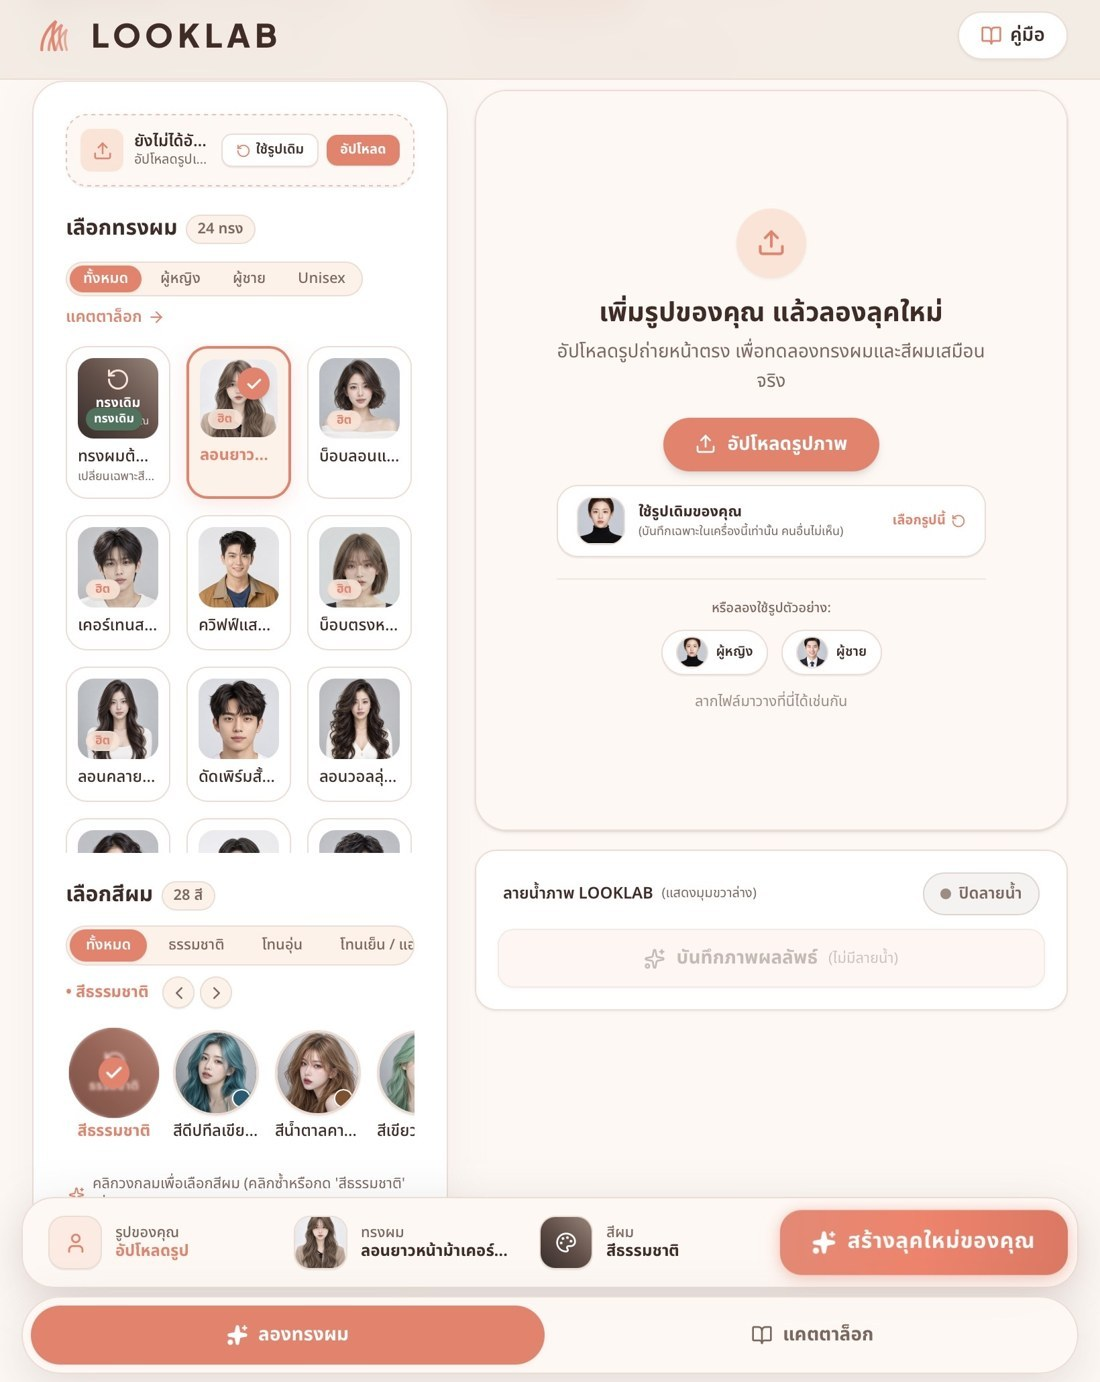
\includegraphics[width=\textwidth]{images/looklab_upload.jpg}
\caption{หน้าหลักก่อนใส่รูป}
\end{subfigure}
\hfill
\begin{subfigure}{0.48\textwidth}
\centering
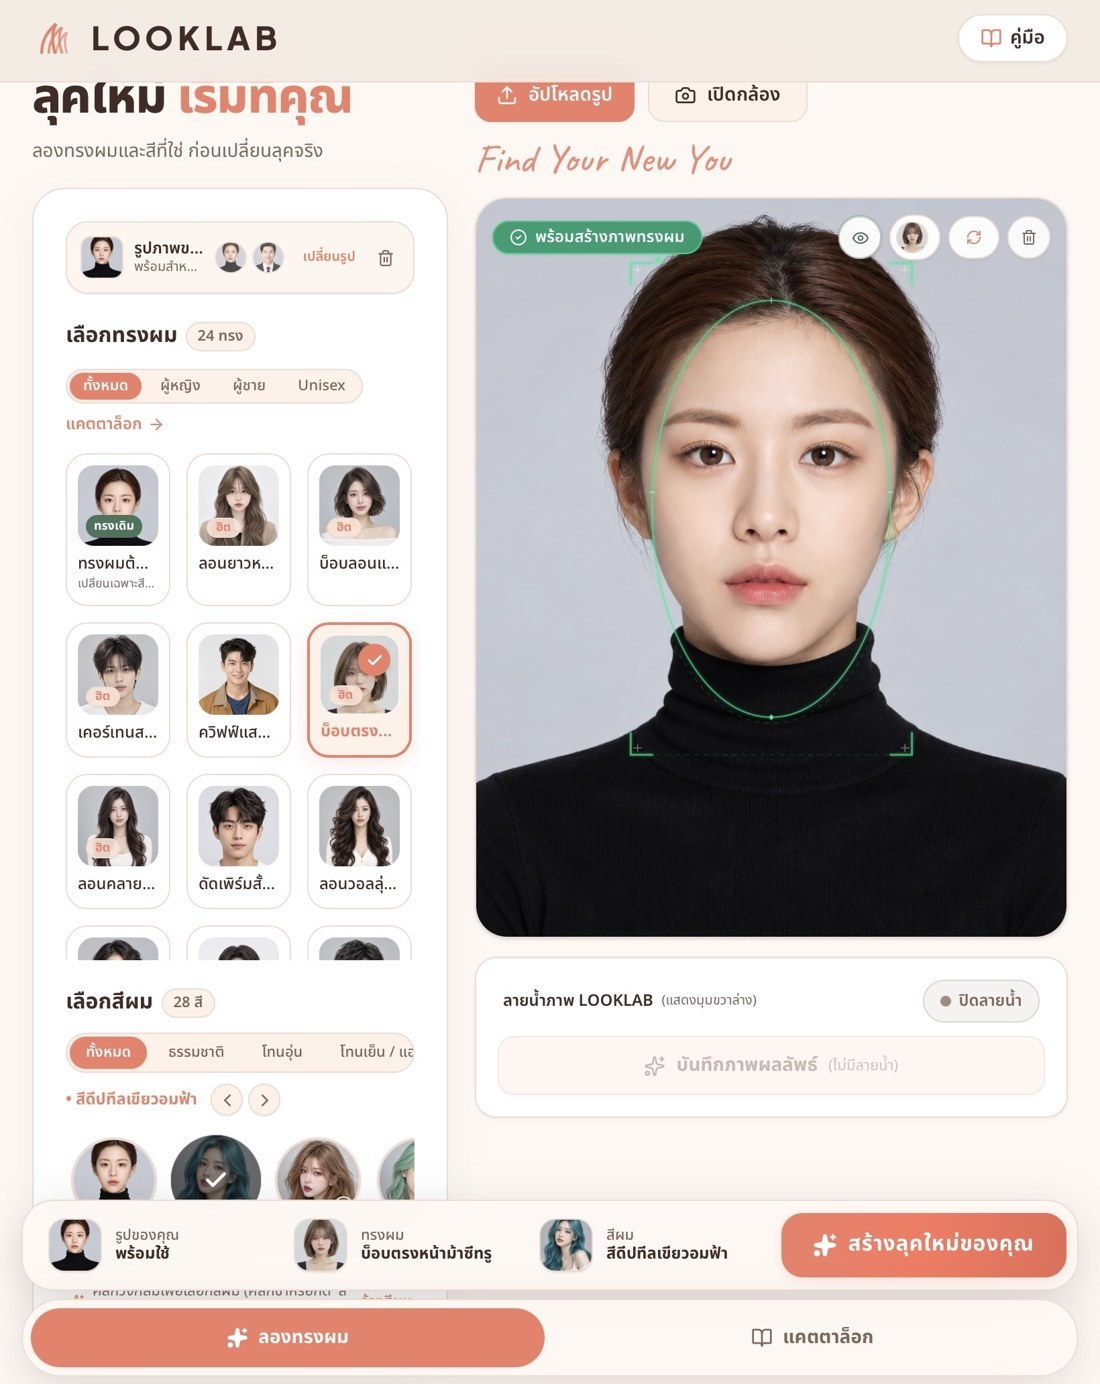
\includegraphics[width=\textwidth]{images/looklab_ready.jpg}
\caption{หลังอัปโหลดรูปและตรวจพบใบหน้า}
\end{subfigure}
\caption{หน้าหลักของเว็บแอปพลิเคชัน LOOKLAB}
\label{fig:web_main}
\end{figure}

\subsection{ตัวเลือกทรงผมและสีผม}

ระบบมีทรงผม 24 แบบ ประกอบด้วยทรงยอดนิยม 23 แบบ เช่น ลอนยาวหน้าม้าเคอร์เทน บ็อบ วูล์ฟคัต ทูบล็อก และควิฟฟ์
และตัวเลือก ``ทรงผมต้นฉบับ'' สำหรับคนที่อยากเปลี่ยนเฉพาะสี
ทรงผมกรองได้ตามกลุ่มผู้หญิง ผู้ชาย และ Unisex
ส่วนสีผมมี 28 สี และมีตัวเลือก ``สีธรรมชาติ'' เพิ่มอีกหนึ่งตัว สำหรับคนที่อยากเปลี่ยนเฉพาะทรง
สีผมกรองได้ตามโทน คือ ธรรมชาติ โทนอุ่น โทนเย็นหรือแอช และแฟชั่นหรือพาสเทล
แต่ละตัวเลือกคือภาพอ้างอิงหนึ่งภาพที่ถูกส่งเข้าโมเดลจริง ไม่ใช่เพียงชื่อทรงหรือรหัสสี
นอกจากนี้ยังมีหน้าแคตตาล็อกที่แสดงทรงผมและสีผมเป็นภาพขนาดใหญ่พร้อมคำอธิบาย ดังภาพที่~\ref{fig:web_catalog}

\begin{figure}[!htbp]
\centering
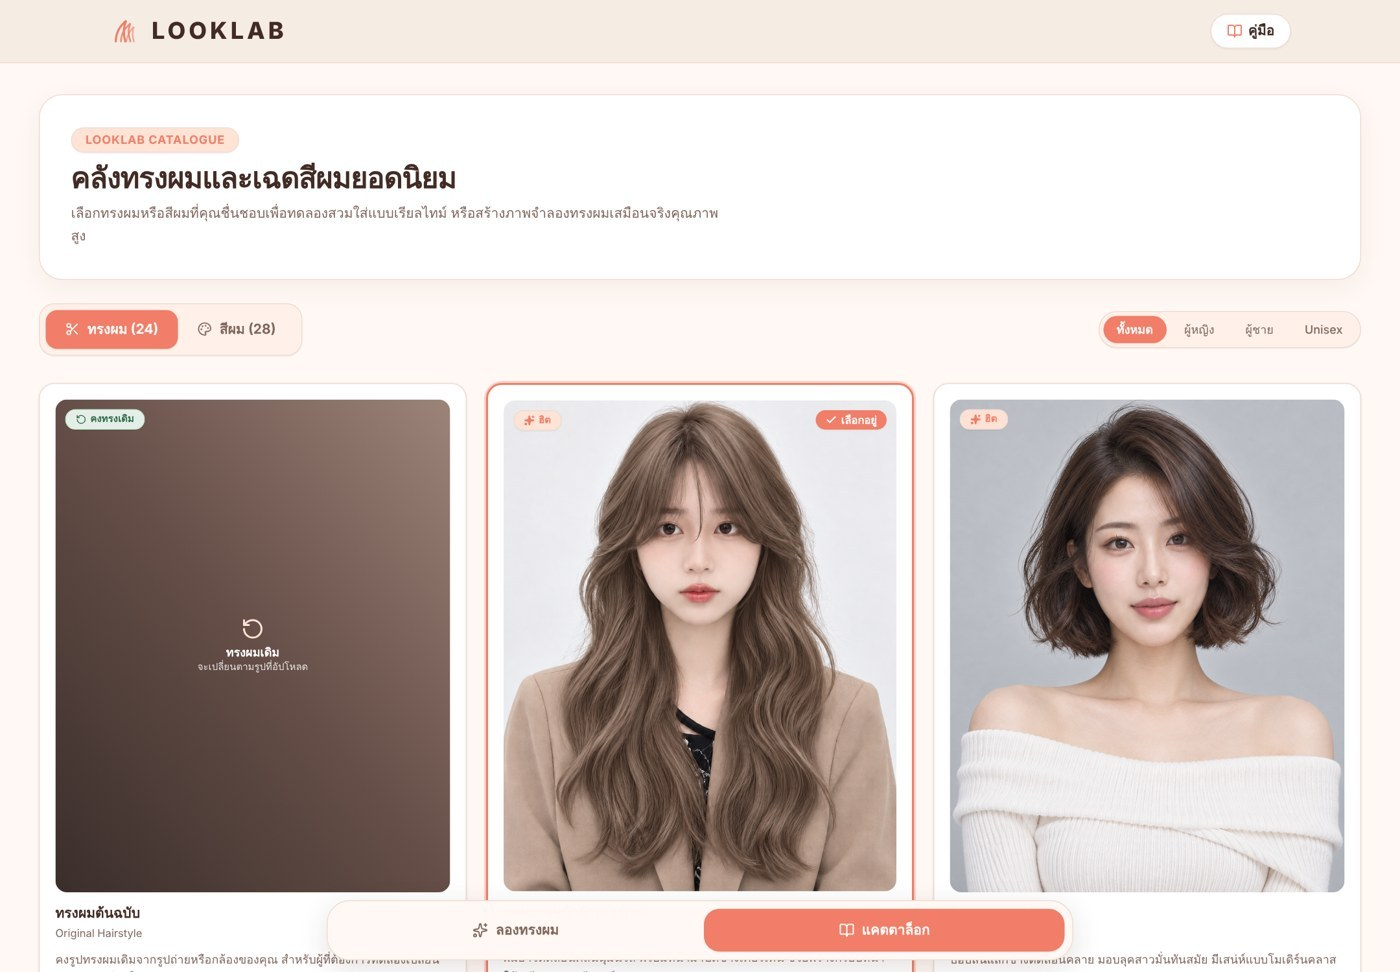
\includegraphics[width=0.8\textwidth]{images/looklab_catalog.jpg}
\caption{หน้าแคตตาล็อกทรงผมและสีผมของ LOOKLAB}
\label{fig:web_catalog}
\end{figure}

\subsection{โหมดกล้องสด}

โหมดกล้องสดออกแบบมาสำหรับคนที่ไม่มีรูปหน้าตรงพร้อมใช้
เมื่อเปิดกล้อง ระบบจะแสดงวงรีนำทางและบอกผู้ใช้ เช่น ``ขยับใบหน้าให้อยู่ตรงกลางกรอบ''
เมื่อใบหน้าอยู่ในกรอบ วงรีจะเปลี่ยนเป็นสีฟ้าและนับถอยหลัง 5 วินาทีก่อนถ่ายภาพอัตโนมัติ
ดังภาพที่~\ref{fig:web_camera} (a)
ภาพที่ถ่ายได้จะถูกส่งไปสร้างทรงผมด้วยโมเดล ซึ่งต้องรอประมาณ 15 วินาที จากนั้นระบบจึงนำผมที่ได้มาซ้อนบนภาพจากกล้อง
โดยใช้จุดสังเกตบนใบหน้าจาก MediaPipe ให้ผมขยับตามศีรษะแบบเรียลไทม์ ดังภาพที่~\ref{fig:web_camera} (b)
ผู้ใช้กดปุ่ม ``บันทึกภาพนิ่ง'' เพื่อเก็บภาพในมุมที่ชอบได้
ภาพในโหมดนี้เป็นการซ้อนภาพผมที่โมเดลสร้างไว้แล้ว ความละเอียดจึงต่ำกว่าโหมดอัปโหลดรูป
ผู้วิจัยจึงแนะนำโหมดอัปโหลดรูปเมื่อต้องการภาพคุณภาพสูงที่สุด

\begin{figure}[!htbp]
\centering
\begin{subfigure}{0.48\textwidth}
\centering
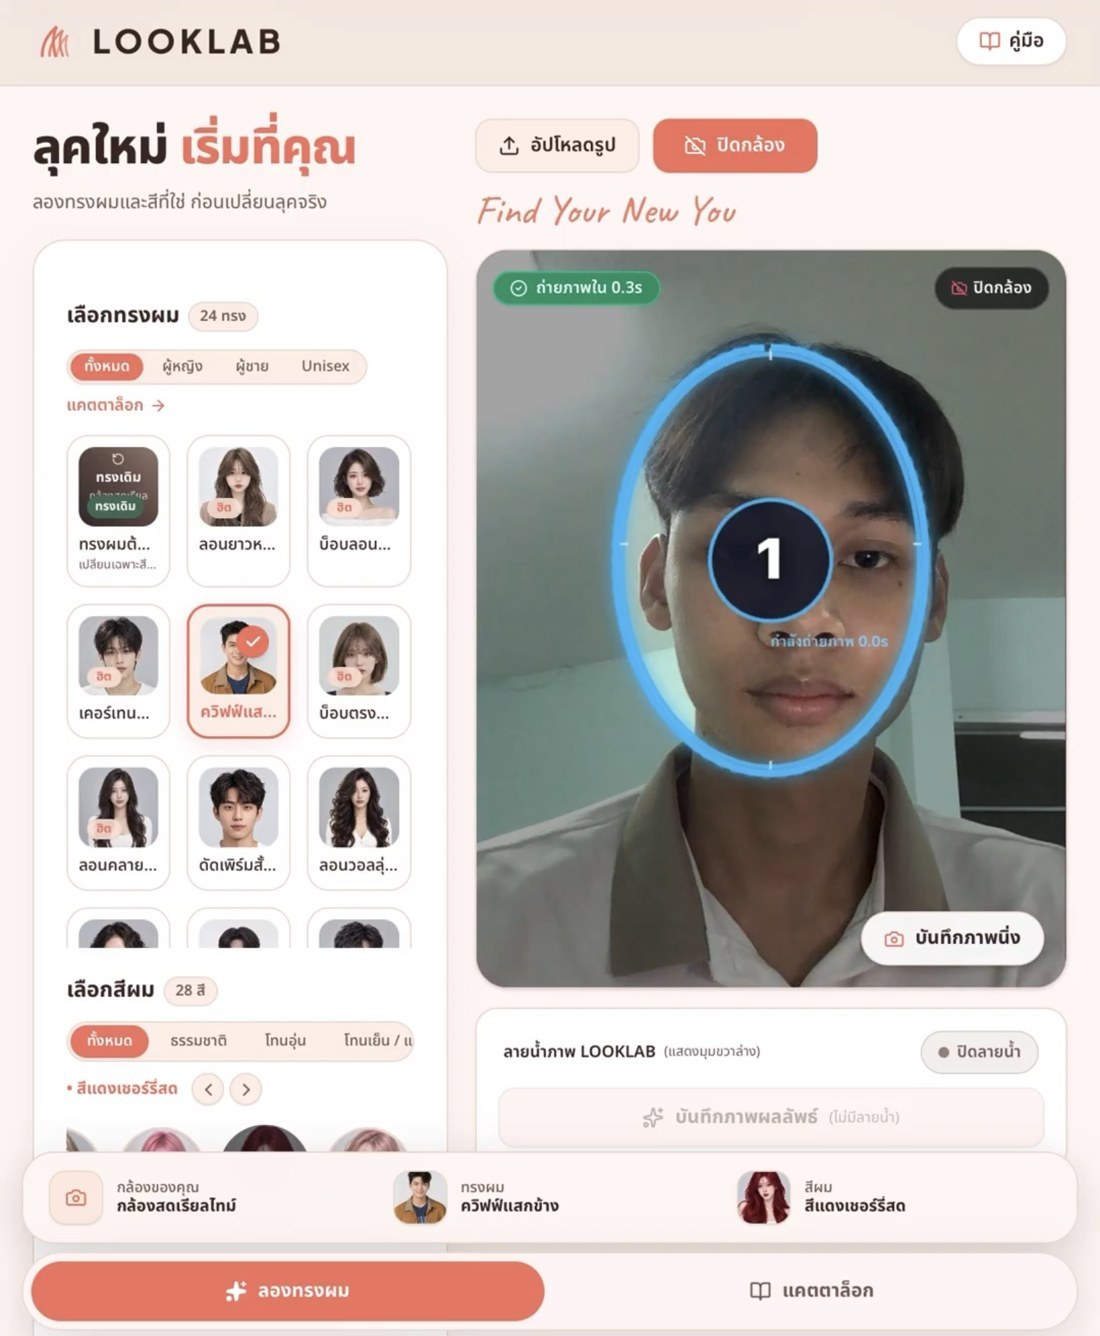
\includegraphics[width=\textwidth]{images/looklab_camera_capture.jpg}
\caption{นับถอยหลังก่อนถ่ายภาพ}
\end{subfigure}
\hfill
\begin{subfigure}{0.48\textwidth}
\centering
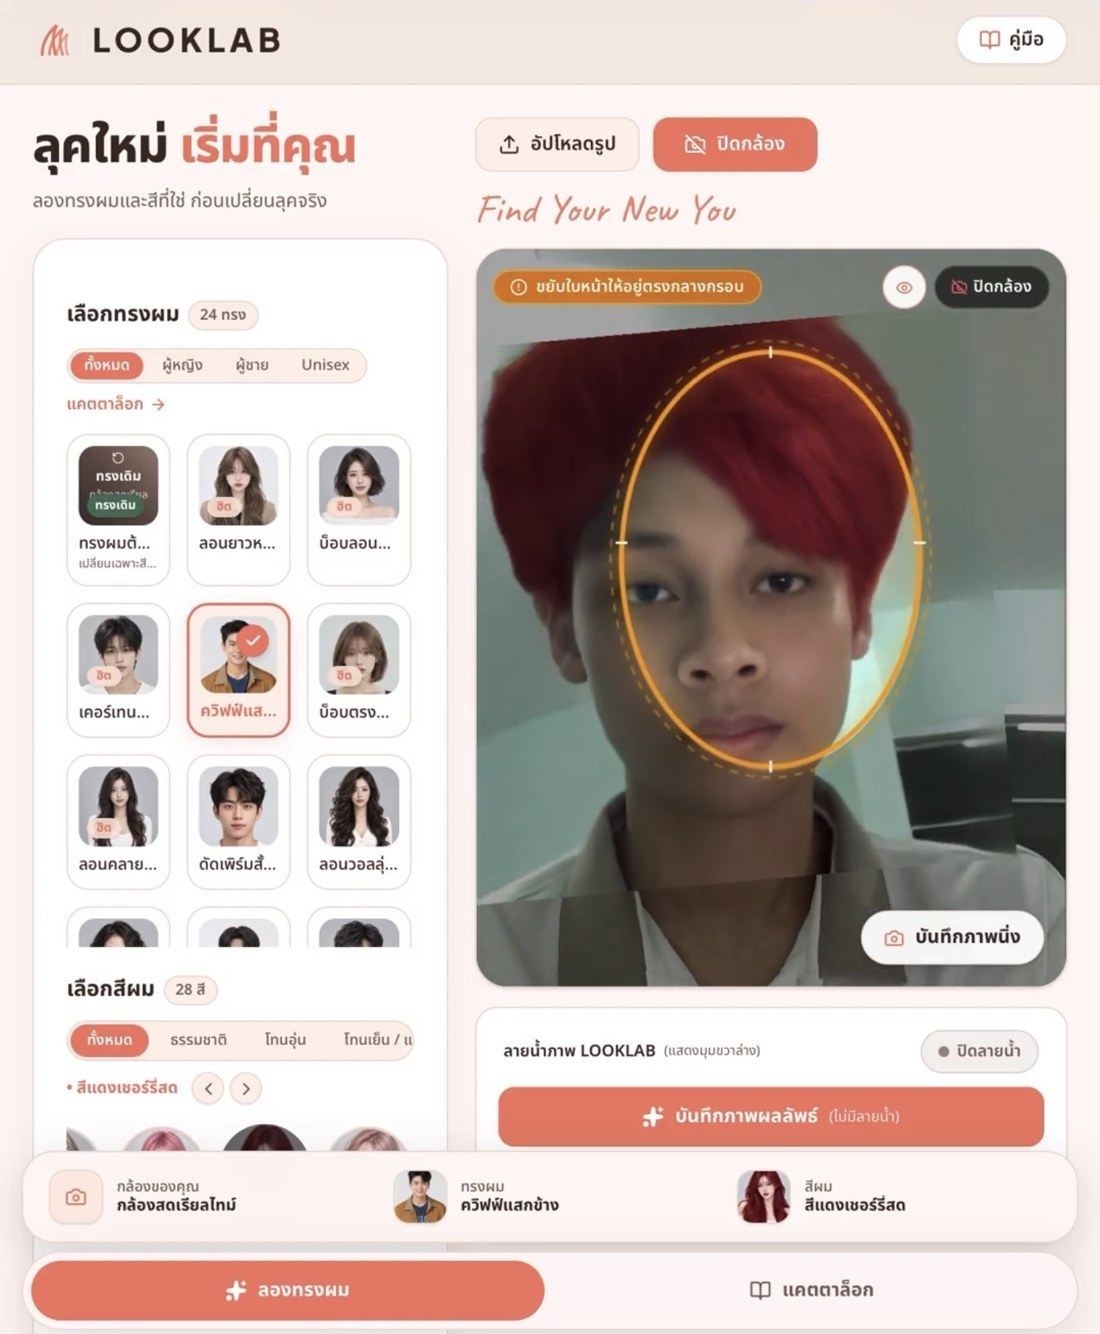
\includegraphics[width=\textwidth]{images/looklab_camera_ar.jpg}
\caption{ทรงผมใหม่ขยับตามใบหน้าแบบเรียลไทม์}
\end{subfigure}
\caption{โหมดกล้องสดของ LOOKLAB}
\label{fig:web_camera}
\end{figure}

\subsection{หน้าผลลัพธ์และแบบสอบถาม}

เมื่อสร้างภาพเสร็จ ภาพผลลัพธ์จะแสดงในพื้นที่เดิม พร้อมแถบเลื่อนเปรียบเทียบก่อนและหลัง (Before/After)
ดังภาพที่~\ref{fig:web_result} (a) ผู้ใช้เลื่อนเส้นกลางไปทางซ้ายหรือขวาเพื่อดูความต่าง
หรือสลับไปดูภาพผลลัพธ์เต็มภาพ และกดขยายเต็มจอได้
ด้านล่างมีปุ่มบันทึกภาพลงเครื่อง ซึ่งเลือกได้ว่าจะใส่ลายน้ำ LOOKLAB หรือไม่
และมีปุ่มเปิดแบบสอบถามประเมินผลลัพธ์

แบบสอบถามในภาพที่~\ref{fig:web_result} (b) แสดงภาพ 4 ภาพเรียงกันก่อนเสมอ
คือ รูปต้นฉบับ ภาพอ้างอิงทรงผม ภาพอ้างอิงสีผม และภาพผลลัพธ์ เพื่อให้ผู้ใช้ตอบโดยเห็นภาพจริงอยู่ตรงหน้า
มุมขวาบนแสดงเวลารอผลลัพธ์จริงที่ระบบจับไว้ จากนั้นผู้ใช้เลือกช่วงอายุ
และให้คะแนน 1--5 ดาวใน 6 ข้อ ตามตารางที่~\ref{tab:app_web} ในภาคผนวก~ข
ผลการทดลองใช้งาน 100 ครั้งในบทที่ 4 มาจากแบบสอบถามนี้

\begin{figure}[!htbp]
\centering
\begin{subfigure}{0.48\textwidth}
\centering
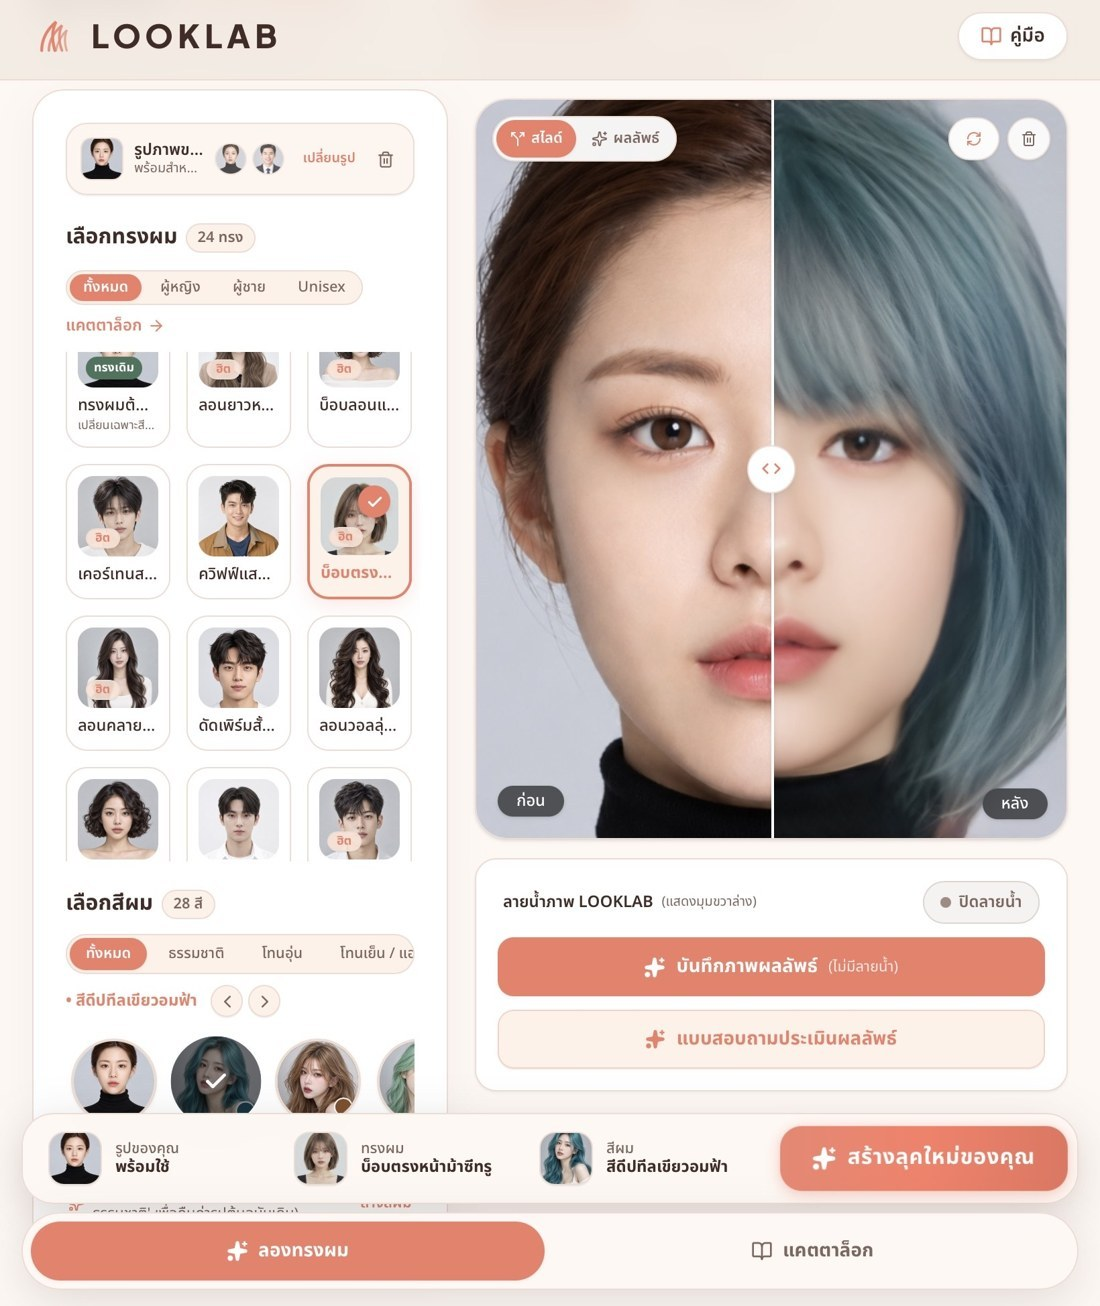
\includegraphics[width=\textwidth]{images/looklab_result.jpg}
\caption{เปรียบเทียบก่อนและหลัง}
\end{subfigure}
\hfill
\begin{subfigure}{0.48\textwidth}
\centering
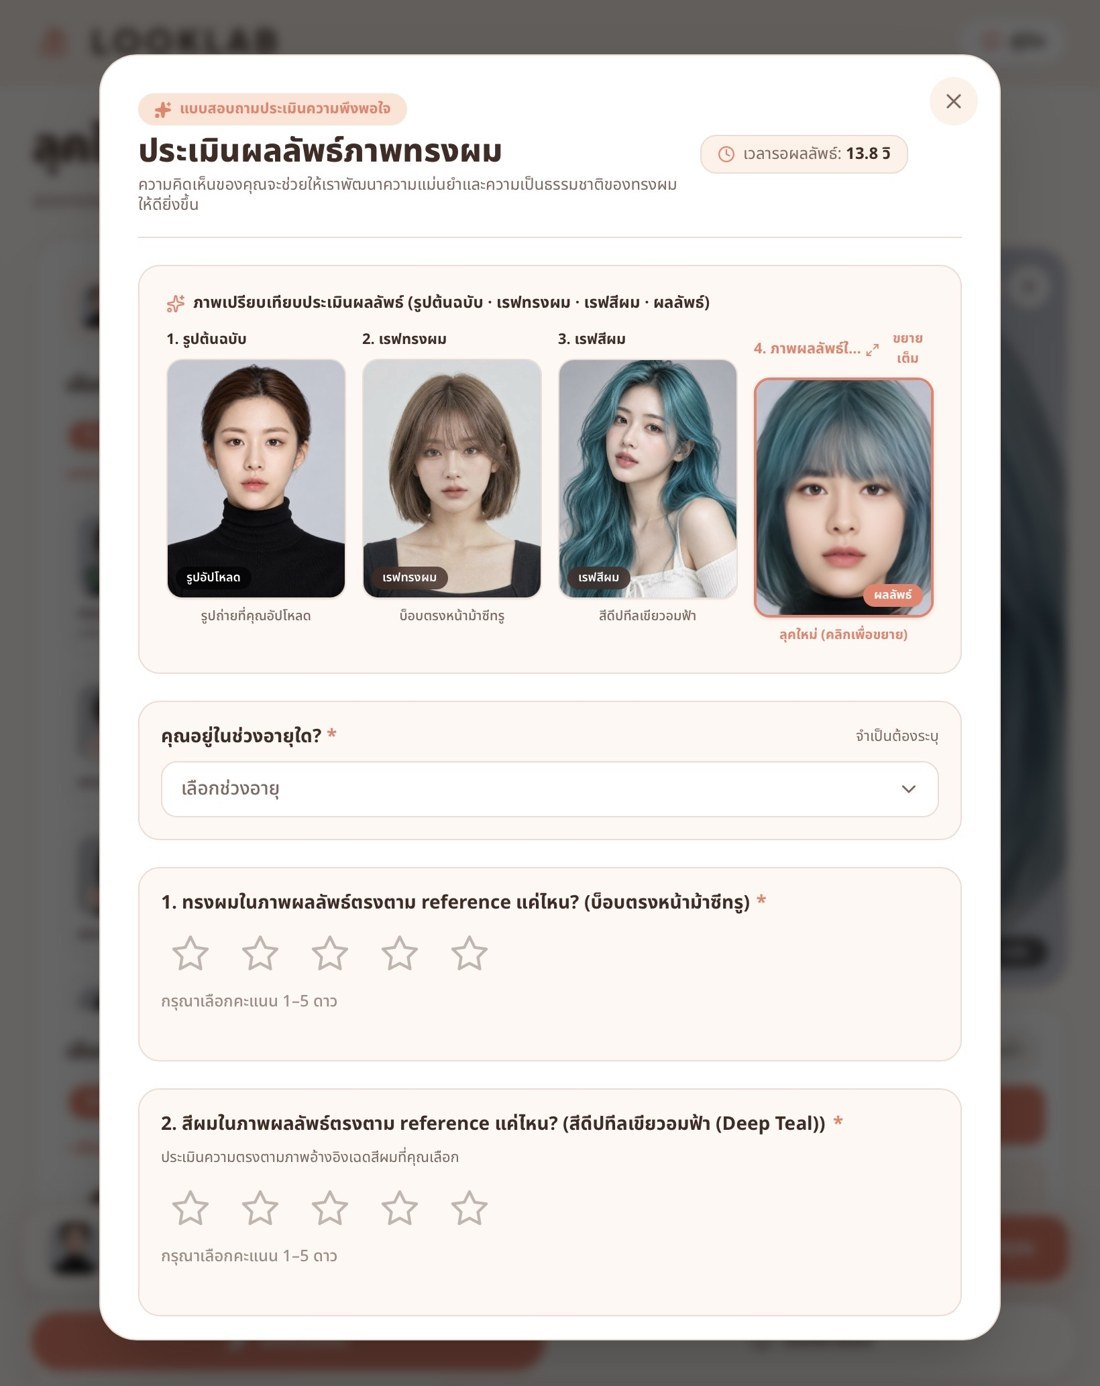
\includegraphics[width=\textwidth]{images/looklab_feedback.jpg}
\caption{แบบสอบถามประเมินผลลัพธ์}
\end{subfigure}
\caption{หน้าผลลัพธ์และแบบสอบถามของ LOOKLAB}
\label{fig:web_result}
\end{figure}


\section{ข้อควรระวังในการตีความและรายละเอียดการคำนวณ}

แม้ทั้งสองโมเดลใช้ฟังก์ชันสูญเสียหลักชุดเดียวกัน แต่ค่าสูญเสียไม่ได้เหมือนกันทุกส่วน
HairFastGAN มีการวัดที่ภาพกลาง (Deep Supervision) และค่าสูญเสียยึดรหัส (Latent Anchor) เพิ่มเติม
และภาพอ้างอิงของ $L_{detail}$ ก็ต่างจาก Barbershop-FT
จึงไม่ควรนำขนาดหรืออัตราการลดของค่าสูญเสียรวมมาเปรียบเทียบความสามารถของสองโมเดลโดยตรง
แต่ควรเปรียบเทียบจากตัวชี้วัดของผลลัพธ์บนข้อมูลชุดเดียวกัน

รายละเอียดการคำนวณในโค้ดมีดังนี้ ภาพทุกภาพถูกปรับค่าให้อยู่ในช่วง 0--1 ก่อนคำนวณ
$E_L$ และ $E_{ab}$ ใช้เปอร์เซ็นไทล์ 9 ค่า (10, 20, \ldots, 90) ของพิกเซลผมด้านใน
โดย $E_{ab}$ เป็นค่าเฉลี่ยรวมของช่อง $a$ และ $b$
ส่วน $L_{protect}$ เฉลี่ยผลต่างของทั้ง 3 ช่องสี RGB
$L_{detail}$ แปลงภาพเป็นความสว่าง แล้วปรับค่าในหน้าต่าง $9 \times 9$ พิกเซลให้มีค่าเฉลี่ย 0 และความแปรปรวน 1
จากนั้นหา MAE เทียบกับภาพอ้างอิงเฉพาะพิกเซลผมด้านใน ที่ความละเอียด 256 และ 512 พิกเซล
ส่วน $L_{shape}$ ใช้ BCE แบบถ่วงดุลและ Dice ที่บวก 1 ตามสมการที่~(\ref{eq:l_shape})

ในการประเมินโดยผู้ใช้ หน่วยของการวิเคราะห์คือบุคคล 41 คน
ส่วน 164 รายการคือจำนวนภาพที่บุคคลเหล่านี้ประเมิน (คนละ 4 ภาพ) ไม่ใช่ผู้เข้าร่วม 164 คน
การหาช่วงความเชื่อมั่นจึงสุ่มบูตสแตรปในระดับบุคคล และเก็บคะแนนที่จับคู่กันของแต่ละคนไว้ด้วยกัน
ส่วนข้อมูลจากเว็บ 100 ครั้งคือจำนวนครั้งที่ใช้งานและตอบแบบประเมิน ซึ่งผู้ใช้หนึ่งคนอาจใช้งานมากกว่าหนึ่งครั้ง
